\chapter{排序学习}\label{chapt:l2r}

互联网的蓬勃发展,尤其是社交网络的诞生,一改往日“信息匮乏”的局面,大数据时代已经来临。搜索引擎是网络用户从海量数据中查找信息的主要入口,因此,如何根据用户的检索请求,迅速地准确定位到相关信息源(如网页、文档、音频、视频、图片等),是搜索引擎能否为用户认可,能否吸引用户的重要标准,而搜索核心环节就是排序:将搜索内容以列表的形式,按照相关程度从高到低展现给用户。

传统的搜索排序主要基于手工构造的模型,计算文档与检索词之间的相关程度。传统的排序模型大致可分为两种类型,基于链接分析的模型,如PageRank\cite{brin1998anatomy,page1999pagerank}, HITS\cite{kleinberg1999authoritative},SALSA\cite{lempel2000stochastic,lempel2001salsa};基于内容分析的模型,如向量空间模型\cite{salton1975vector},BM25\cite{robertson2009probabilistic}。目前影响网页排名的因素有上千种,传统排名算法面对这种复杂局面,存在以下几个方面的不足:(1)考虑的影响因素比较单一;(2)对多个影响因素的融合能力较差;(3)使用时不够灵活;(5)对复杂模型的参数调整比较困难。
\begin{figure}[htbp]
  \centering
  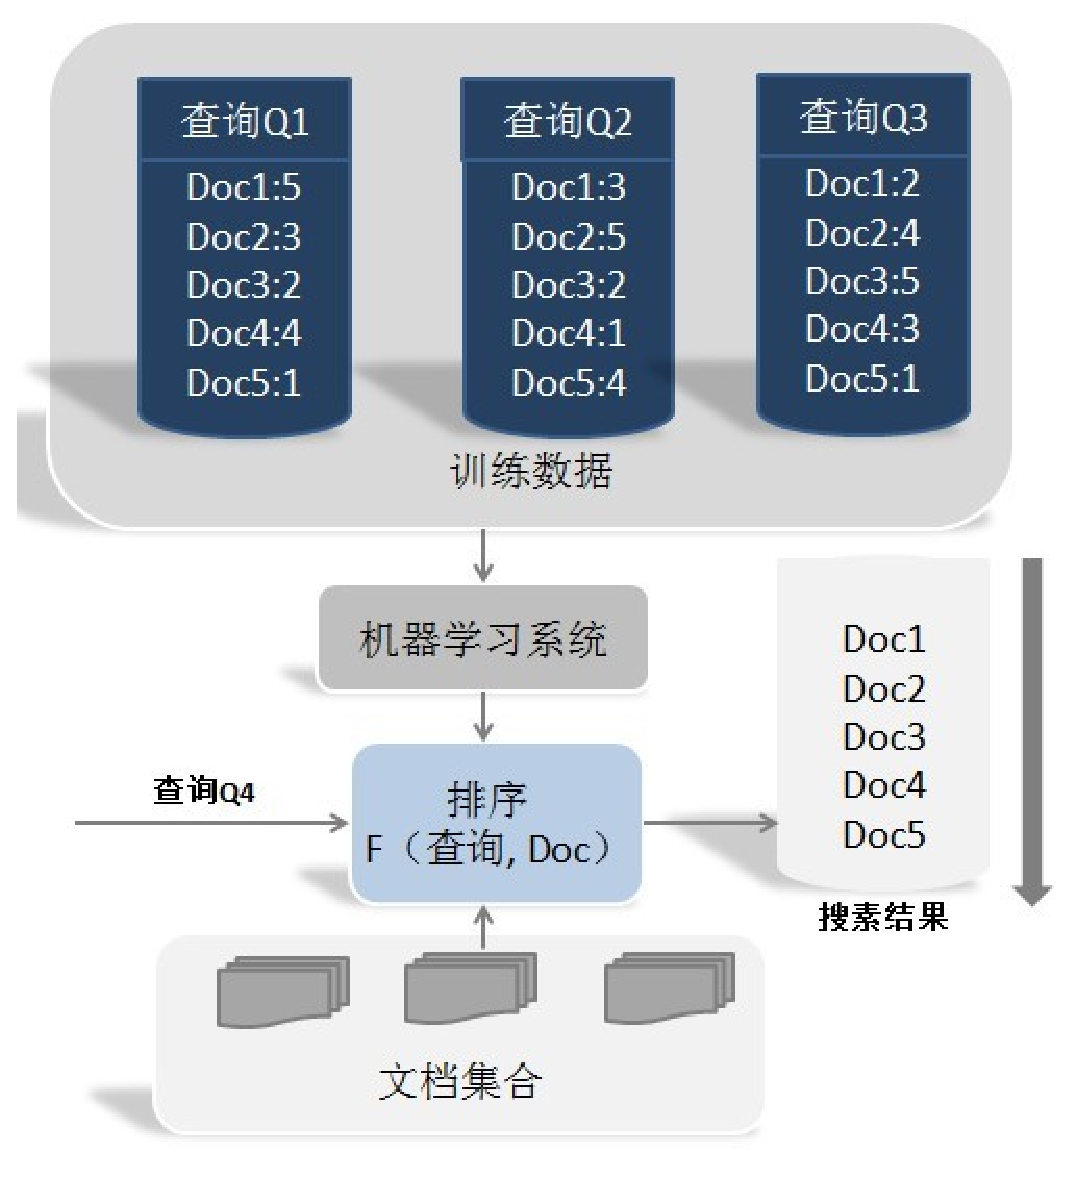
\includegraphics[width=0.5\textwidth,height=8cm]{figures/l2r.eps}
  \caption{排序学习框架}\label{fig:l2rframwork}
\end{figure}

排序学习\cite{trotman2005learning,liu2009learning}可以在一定程度上克服传统排序的缺点。它结合机器学习的方法,可以自动地从训练数据集中学习排名函数。序列型排序学习方法是目前最直接,也是表现最好的一类排序学习方法。排序学习是一种典型的监督学习方法,需要利用带有人工标记的标准数据集训练模型。数据集一般包含多个检索词,每个检索词存在多个关联文档,每个文档由一个多维特征向量(每个特征都可以单独作为一个排名函数,如PageRank,TF*IDF等)表示,相应地,每篇文档都有一个人工标记的相关等级,反映文档同检索词的相关程度。

\ornamento
\section{背景介绍}
排序学习方法是一种有效的排名技术,借鉴机器学习的监督学习方法,通过优化损失函数,从训练数据集中学习一个排名函数。排序学习是一个较新的研究方向,在过去十年间发展迅速,已经被成功地应用到网页搜索、机器翻译和系统推荐等领域\cite{liu2009learning}。

Liu\cite{liu2011learning}和Li\cite{li2011learning}根据输入空间、输出空间、模型假设和损失函数的不同,将排序学习方法划分为三类:逐点型(Pointwise)、序对型(Pairwise)、序列型(Listwise)。

逐点型排序学习方法将排名问题转化为传统的分类、(有序)回归问题,根据成熟的分类和回归算法,使用分类错误率或者均方差构建损失函数,训练排名函数。比如,Crammer和Singer\cite{crammer2001pranking}提出的PRank算法,通过训练一个感知器模型,把训练样本映射到一个全序集。

序对型排序学习算法的训练数据是成对的样本,根据模型假设预测序对的偏好关系,结合真实相关等级,构造序对损失函数,模型训练的目标即最小化序对损失函数。典型的序对型排序学习算法有:Herbrich等人\cite{herbrich1999large}将排序问题转化为序对型分类问题,基于支持向量机(Support Vector Machine, SVM)提出RankingSVM 算法;Freund等人\cite{freund2003efficient}根据提升(Boosting)技术,将用于分类的经典算法AdaBoost应用到序对型排序学习问题,提出了RankBoost算法;Burges等人\cite{burges2005learning}根据神经网络(Artificial Neural Network, ANN)的进化学习理论,辅以梯度下降的优化方法调整模型参数,训练排序模型,提出RankNet 算法;由于标准评价指标是非平滑不可微的,无法直接优化,Burges等人\cite{burges2007learning}分析交换序对文档名次引发的成本变化,直接定义损失函数的梯度
(Lambda),改进RankNet算法引入LambdaRank。

序列型排序学习方法直接将整个样本集合作为学习对象,根据模型的预测结果和真实排名列表构建出序列型损失函数,通过优化序列型损失函数训练排序模型。比如,2007 年Xu和Li\cite{xu2007adarank}基于Boosting技术,以单个特征作为备选弱排名函数,提出一种高效的学习算法——AdaRank。同年,Cao等人\cite{cao2007learning}认为在训练过程中,RankNet算法使用的交叉熵损失函数降低的同时却无法保证标准度量指标相应地提升,于是提出一种基于概率模型的排序模型ListNet。ListNet是RankNet的一种序列型扩展。Qin等人\cite{qin2008query}提出的RankCosine算法是基于余弦损失函数,使用梯度下降法在神经网络上训练模型。Xia等人\cite{xia2008listwise}于2008年提出的ListMLE算法同ListNet类似,都是基于Plackett-Luce概率模型、神经网络技术和梯度下降法训练排名函数,但是ListMLE根据真实排名列表,假设列表中各个位置服从指数概率分布,并根据最大似然估计,定义似然损失函数。

由于衡量排序性能的标准评价指标需要考虑文档位置信息,因此是非平滑的不可微函数,序列型排序学习方法“直接”优化目标多是对性能指标作平滑近似或者通过寻找性能评价指标的平滑上界,间接地进行优化。如Taylor等人\cite{taylor2008softrank}提出的SoftRank算法根据模型的预测结果,使用SoftNDCG近似文档的排名分布,属于平滑近似方法。Yue等人\cite{yue2007support}提出的SVM\textsuperscript{MAP}模型和Chakrabarti等人\cite{chakrabarti2008structured}推出的SVM\textsuperscript{NDCG}模型分别对标准评价指标MAP和NDCG估计出其平滑上界,均属于确定平滑上界的方法。

序列型排序学习方法实际上是直接优化性能评价指标,相比逐点型、序对型排序学习方法而言,训练过程较为直观,损失函数同性能评价指标之间的一致性更强,而且不易受检索词关联文档数目差异的影响。序列型排序学习方法内在地要优于序对型排序学习方法。

\section{研究团队}
目前研究排序学习的主要团队有微软亚洲研究院(如Hang Li,Tie-Yan Liu等),微软Bing搜索已经使用RankNet算法,但更偏重于理论证明。
俄罗斯的Yandex研究团队在2009年Yahoo!举办的Learning to Rank Challenge中取得不错的名次,而且据说Yandex 搜索引擎已经开始使用排序学习训练的模型改善搜索质量。据称,Yandex 从2009年开始使用一种新的机器学习模型MatrixNet,融合了上千种搜索因素,极大地改善搜索的质量。Yandex还举办了Internet Mathematics 2009竞赛。2002年前后,AltaVista首先使用Boosted Tree Regression构建基于排序学习的排名系统,系统上线后,排名第一的网页点击率有明显提升。百度网页搜索于2011年左右引入机器排序学习,并发布排序学习算法工程师的招聘通知。Google对排序学习的兴趣不高;Cuil的CEO认为由机器学习的模型没有人工构造的模型健壮。

数学界对排序问题的兴趣逐渐增加。Belgian Mathematical Society \& National Committee of Mathematics 联合组织了2008年10月15日的
\href{http://nalag.cs.kuleuven.be/research/workshops/ranking/}{The Mathematics of Ranking};美国数学学会(American Institute of Mathematics)于2010年8 月16日-20日承办的\href{http://www.aimath.org/ARCC/workshops/mathofranking.html}{Workshop on the Mathematics of Ranking}。

排序学习的研究团队主要包括:
\begin{itemize}
\item \href{http://www.cse.iitb.ac.in/\~soumen/}{Soumen Chakrabarti's group}
\item \href{http://olivier.chapelle.cc/index.html}{Olivier Chapelle's group}
\item \href{http://www.cs.cornell.edu/People/tj/}{Thorsten Joachims's group}
\item \href{http://l2r.cs.uiuc.edu/~cogcomp/projects.php}{Dan Roth's group}
\item \href{http://www.cc.gatech.edu/\~zha/}{Hongyuan Zha's group}
\item \href{http://research.microsoft.com/\~cburges/}{Web Learning Group, Microsoft Research}
\item Information Retrieval and Mining Group, Microsoft Research Asia
\item Yandex's lab, Yahoo! Research Center
\item \href{http://ir.dlut.edu.cn/}{大连理工大学信息检索研究室}
\item \href{http://kdd.nankai.edu.cn/IIP/jsp/index/index.jsp}{南开大学智能信息处理实验室}
\end{itemize}

\section{PRank}
2001年,Koby Crammer与Yoram Singer\cite{crammer2001pranking}提出PRank(Perceptron Rank)排名方法,将检索词-文档对作为训练样本,每个训练样本对应一个相关等级。PRank 的目标是训练多个平行的分隔超平面(感知器)将样本正确的区分开,根据PRank 训练得到的排序模型可以表示为如下形式的判定函数:
\begin{equation}\label{eq:pranking}
    f(x) = \min \limits_{r\in \{1,2,\ldots, k\}}\{\omega^T x - b_r < 0\}
\end{equation}
其中,参数$\omega$表示分隔超平面的法向量,$b_r$表示分隔超平面的截距,$r=1,2,\ldots,k$,并且满足$b_1 < b_2 < \cdots < b_{k-1} < b_k = + \infty$。

在训练过程,PRank同时调整法向量与截距组,从而减少预测排名的损失,并由模型的保序性与误差有界性保证收敛性。

\section{RankSVM}
2002年,Thorsten Joachims\cite{joachims2002optimizing}基于SVM技术,提出RankSVM,它是一个经典的序对型排序学习模型。RankSVM根据样本真实相关等级对样本序对重新标记,比如对样本空间$\mathcal{X}$中任意关联于相同检索词的样本$x_i$ 与$x_j$,构成序对$z_{ij} = (x_i,x_j)$,如果$y_i > y_j$,则标记$z_{ij}$ 的类标为$+1$,否则就标记为$-1$。 从本质上来看,RankSVM是将排序问题转化为二元分类问题,并使用成熟的SVM技术予以解决。

假设排名函数是线性模型
\[
    f(x) = \omega^T x,
\]
RankSVM根据偏好序对集合$\mathscr P = \{(i,j)| y_i > y_j, x_i,x_j \in \mathcal{X}\}$,构建一个二次优化模型:
\begin{equation}\label{eq:ranksvm}
  \begin{array}{ll}
    \min \limits_{\omega,\xi} & \frac{1}{2}\omega^T\omega + C\sum\limits_{(i,j)\in \mathscr P} \xi_{ij}\\
    \textit{s.t.}& \omega^T(x_i - x_j) > 1- \xi_{ij}\\
    & \xi_{ij} \ge 0,\forall (i,j)\in \mathscr P\\
  \end{array}
\end{equation}
目标函数中,$\omega^T\omega$反映了超平面的间隔,$\xi_{ij}$表示松弛变量。

RankSVM模型能够利用复杂特征进行排序,并取得良好的排序效果,但是它存在一个致命的缺陷:模型训练时间长。由于模型是序对型,对于大小为$n$的训练集,组成大约$n^2$个样本序对,给训练速度带来巨大的负面影响。对此,\cite{joachims2006training,airola2011training}提出改进,降低训练复杂度。

由于RankSVM采用单一的判别函数对所有检索词排序,不具有普遍适用性,对其排序性能构成负面影响。为此,\cite{jung2011ensemble}基于RankSVM,对每个检索词训练一个基本排序模型,使用前向分步加法模型集成基本排序模型。假设训练集包含$m$个检索词$\mathcal{S} = \{(x^{(i)}, y^{(i)})\}_{i = 1}^m$,其中,$x^{(i)} = \{x_1^{(i)},\ldots, x_{n_i}^{(i)}\}$表示第$i$个检索词的关联文档特征向量集合,$n_i$表示关联文档的数目,$x_j^{(i)}\in \mathbb R^d$表示第$j$个关联文档的特征向量,$y^{(i)} = \{y_1^{(i)},\ldots, y_{n_i}^{(i)}\}$表示与$x^{(i)}$对应的相关等级标记。验证集是$\mathcal{V} = \{(x^{(k)}, y^{(k)})\}_{k = 1}^K$,其中$K$ 表示验证集中包含的检索词总数。具体步骤如下:
\begin{enumerate}[(1)]
  \item 选择$(x^{(i)}, y^{(i)}), i = 1,\ldots, m$作为独立的训练数据集,在每个独立训练集上应用RankSVM训练排序模型,构成$m$个基本排序模型$\{f^{(i)}\}_{i = 1}^m$。
  \item 对$\{f^{(i)}\}_{i = 1}^m$基本模型重新排列,构成一个有序队列$\pi$,并选择第一个排序模型记为$f$,计算$f$在验证集上的平均性能$mp$,将$f$添加至候选排序模型集合$\mathcal{F} = \{f\}$。
  \item 从有序队列$\pi$中选取第二个模型$f'$,如果$f + f'$在验证集上的平均性能$mp' \ge mp$,则更新$f = f + f', mp = mp'$,将$f'$添加到排序模型集合$\mathcal{F} = \{f, f'\}$;如果$f + f'$ 的平均性能$mp' < mp$,则选择$\pi$下一个模型,直至遍历尽全部基本排序模型。
  \item 将候选排序模型集中所有候选排序模型加和,得到最终排序模型$F$,并计算$F$在验证集上的平均性能$mp_{\max}$。
  \item 重复执行以上三个步骤$T$次,将每次迭代获取的最终候选排序模型在验证集上的平均性能降序排列,选择处于中间位置的$mp_{\max}$对应的排序模型作为学习得到的最终排序模型。
\end{enumerate}

\cite{jung2011ensemble}提出的模型时间复杂度为$\complex((M/m)^2 \times m) = \complex(M^2/m)$相比RankSVM 的$\complex(M^2)$ 提升了$m$ 倍,易于训练大规模数据,其中$M$表示训练数据集中样本总量。此外,由于每次选择模型时仅仅保留对平均性能有贡献的基本模型,因此排序的平均精度有所提升。

\section{IR-SVM}
\cite{cao2006adapting}Adapting Ranking SVM to Document Retrieval

\section{SVM-MAP}
\cite{yue2007support}A support vector method for optimizing average precision

\section{RankNet}
2005年,微软研究院的Chris Burges等人\cite{burges2005learning}在第22届国际机器学习会议上提出RankNet算法。它是一种典型的序对型排序学习方法,以神经网络生成模型的假设空间,以样本序对的真实相关等级构建偏好概率模型和交叉熵损失函数,利用BP算法更新网络权值、优化调整模型参数。RankNet算法是一种新颖有效的排序模型,据信已纳入微软Bing搜索引擎的核心搜索框架。

\subsection{交叉熵损失函数}
给定任意一组文档对$d_i,d_j$,它们的真实相关等级分别是$y_i,y_j$,对两者的相关等级差值$y_i-y_j$应用Logistic变换,表示“人们偏好$d_i$甚至$d_j$的概率”:
\begin{equation}
    p(d_i\succ d_j) = p_{ij} = \frac{1}{1+e^{-(y_i-y_j)}}
\end{equation}
文档$d_i$的等级与$d_j$的等级差值越大,则人们偏好$d_i$甚于$d_j$的可能性越大。偏好概率关于等级差值呈S形分布,当$y_i=y_j$,两个文档相关等级相同时,偏好概率为$p_{ij}=0.5$,表现出的不确定最强。当$y_i>y_j$时,偏好概率大于0.5,断定“文档$d_i$比文档$d_j$更相关”的可信性更高;反之,偏好概率小于0.5,断言“文档$d_j$ 比文档$d_i$更相关”更可信。

根据真实偏好概率的定义可以推知
\begin{equation}
    y_i-y_j=\log \frac{p_{ij}}{1-p_{ij}}
\end{equation}
对任意的三个文档$d_i,d_j,d_k$,由等式$y_i-y_k=(y_i-y_j) + (y_j - y_k)$,我们得到下面形式的关系式
\begin{equation}
    p_{ik} = \frac{p_{ij}p_{jk}}{p_{ij}p_{jk} + (1-p_{ij})(1-p_{jk})}
\end{equation}
可以证明:对于有限的训练样本,仅仅计算相邻样本对的偏好概率,便可唯一确定任意一个训练样本对的偏好概率。
\begin{theorem}
给定一组样本$x_i,~i=1,\ldots,n$,自然数集合$\{1,\ldots,m\}$的排列组合$\pi$。任取$\pi$两个相邻位置$(i,i+1)$,记$k=\pi(i),j=\pi(i+1)$,利用Logistic 变换可以计算后验邻接概率$p_{kj}$。给定任意一个邻接概率集合,可以唯一确定任意一个样本对$x_i,x_j$的后验目标概率$p_{ij}$,反之亦然。
\end{theorem}

当~$p_{ij}=p_{jk}=p$~时有关系式
\begin{equation}
    p_{ik} = \frac{p^2}{p^2 + (1-p)^2} = \frac{p^2}{2p^2 - 2p + 1},~~p\in [0,1]
\end{equation}
成立。根据组合概率$p_{ik}$同$p$的关系(见图\ref{fig:preferenceprob}),只有在$p=\{0,0.5,1\}$时,才有组合概率$p_{ik}=p$。当$p<0.5$时,组合概率$p_{ik}<p$;当$p>0.5$时,组合概率$p_{ik}>0.5$。由分析可知,偏好概率模型是一致的。

%在搜索排名算法中,理想的排名系统能够准确地给出用户期望的排名列表,使得排名越靠前的搜索条目与用户的需求越相关,偏好程度更高。假设对于任意一组文档$x_i,x_j,x_k$,统计用户对搜索结果的点击率发现,人们偏好$x_i$甚于$x_j$,偏好$x_j$甚于$x_k$的概率都是$p$,那么,文档$x_i$的排名高于$x_j$的概率也是$p$?

%偏好的传递性

\begin{figure}[htbp]
  \begin{minipage}[t]{0.49\linewidth}
      \centering
      \includegraphics[width=0.9\textwidth]{figures/preferenceprob.eps}
      \caption{偏好概率模型}\label{fig:preferenceprob}
  \end{minipage}
  \begin{minipage}[t]{0.49\linewidth}
      \centering
      \includegraphics[width=0.9\textwidth]{figures/entropyloss.eps}
      \caption{交叉熵损失函数}\label{fig:entropyloss}
  \end{minipage}
\end{figure}

假设排序模型是连续函数$f:\mathbb{R}^m\mapsto \mathbb{R}$,对评分结果经过Logistic函数变换,可用于估计真实偏好概率:
\begin{equation}
    \widetilde{p}_{ij} = \frac{1}{1+e^{-o_{ij}}}
\end{equation}
其中,$o_{ij}=f(\theta,x_i)-f(\theta,x_j)$表示样本序对的预测差值。

排序模型预测结果同真实结果之间的差异可以使用概率分布的交叉熵距离表示,并直接用于度量排序模型在样本序对$(x_i,x_j)$上的预测损失
\begin{equation}
    \begin{array}{lll}
      L_{ij} & = & -\big[p_{ij} \log \widetilde{p}_{ij} + (1-p_{ij}) \log (1-\widetilde{p}_{ij})\big] \\
       & = & p_{ij} \log(1+e^{-o_{ij}}) + (1-p_{ij}) \log(1+e^{o_{ij}}) \\
       & = & \log(1+e^{o_{ij}}) - p_{ij} o_{ij}
    \end{array}
\end{equation}

交叉熵损失函数$L_{ij}$与真实偏好概率$p_{ij}$密切相关(见图\ref{fig:entropyloss}),偏好概率$p_{ij}$取值不同,损失函数随预测差值的变化趋势也不同。当$p_{ij}=0.5$ 时,表明样本序对的真实排名相同,损失函数关于样本序对的预测差值$o_{ij}$对称。当$o_{ij}=0$时损失量最小$L_{ij}=\log 2$,仍大于零。

\subsection{训练}
RankNet算法使用一个三层神经网络表示排序模型
\begin{equation}
    f(\theta,x) = \varphi \Big(b + \sum\limits_{l=1}^h \upsilon_l \phi_l\big(b_l + \sum\limits_{k=1}^m \omega_{kl} x_k\big)\Big)
\end{equation}
其中,输入层有$m$个输入节点,隐藏层有$h$个节点,输出层只有一个输出节点。隐藏层的刺激函数为$\phi_1,\ldots,\phi_h$,输出层的刺激函数$\varphi$,均为Sigmoid函数。$b_1,\ldots,b_h$与$b$都是偏置量。参数$\omega_{kl}$表示第$k$个输入节点到第$l$个隐藏节点的连接权值,$\upsilon_l$则是第$l$个隐藏节点到输出节点的权值。$x_k$表示输入向量$x$的第$k$个元素。

\begin{algorithm}[htbp]
        \caption{RankNet算法}
        \begin{algorithmic}
            \REQUIRE ~~训练集$\{(x_i,x_j),p_{ij},(i,j)\in \mathscr P\}$,学习率$\eta$,迭代次数$T$,初始网络参数$\theta_0$ \\
            \FOR{$t = 1,\dots, T$}
                \FOR{对任意的$(i,j)\in \mathscr P$}
                \STATE
                \begin{enumerate}
                  \item 前向传播:以$(x_i,x_j)$为输入,计算当前网络的输出值
                  \[
                    \begin{array}{l}
                      f_i=f(\theta_{t-1},x_i) \\
                      f_j=f(\theta_{t-1},x_j)
                    \end{array}
                  \]
                  \item 反向传播:使用梯度下降法更新网络参数
                  \[
                    \theta_t = \theta_{t-1} - \eta \nabla L_{ij}
                  \]
                \end{enumerate}
                \ENDFOR
            \ENDFOR
            \ENSURE ~~排序模型$f(\theta_T,x)$
        \end{algorithmic}
\end{algorithm}

RankNet算法使用样本训练集$\{x_i,y_i\}_{i=1}^n$上的偏好序对
\begin{equation}
    \mathscr P = \{(i,j)\mid y_i \ge y_j, i,j=1,\ldots,n\}
\end{equation}
作为网络模型训练样本的索引集,每次训练时从训练集中选取一对样本$(x_i,x_j)$作为输入,通过\textbf{前向传播}(Forward Propagation)在整个网络扩散,产生一对网络输出$(f(\theta,x_i),f(\theta,x_j))$。

假设网络模型的刺激函数都是连续可微的,可以计算网络模型$f(\theta,x)$交叉熵损失函数的梯度
\begin{equation}\label{eq:ranknet-gradient}
    \nabla_{\theta} L_{ij} = \frac{\partial L_{ij}}{\partial o_{ij}} [\nabla_{\theta} f_i- \nabla_{\theta} f_j]
\end{equation}
其中,$f_i=f(\theta,x_i),f_j=f(\theta,x_j)$。根据$f_i$关于$b,\upsilon_l,b_l,\omega_{kl}$的一阶导数
\begin{equation}
    \left\{
    \begin{array}{l}
      \nabla_b f_i = \varphi'(\theta,x_i) \equiv \nabla_1^{(i)} \\
      \nabla_{\upsilon_l} f_i = \varphi'(\theta,x_i) \phi_l(b_l,\omega,x_i) = \nabla_1^{(i)}  \phi_l(b_l,\omega,x_i) \\
      \nabla_{b_l} f_i = \varphi'(\theta,x_i) \upsilon_l \phi'_l(b_l,\omega,x_i) = \nabla_1^{(i)} \upsilon_l \phi'_l(b_l,\omega,x_i) \equiv \nabla_2^{(i)} \\
      \nabla_{\omega_{kl}} f_i = \varphi'(\theta,x_i) \upsilon_l \phi'_l(b_l,\omega,x_i) x_{ik} = \nabla_2^{(i)} x_{ik}
    \end{array}
    \right.
\end{equation}
可以推导得到损失函数$L_{ij}$的梯度:
\begin{equation}
    \left\{
    \begin{array}{l}
      \nabla_b L_{ij} = L'_{ij} \big[\nabla_1^{(i)} - \nabla_1^{(j)}\big]\\
      \nabla_{\upsilon_l} L_{ij} = L'_{ij} \big[\nabla_1^{(i)}  \phi_l(b_l,\omega,x_i) - \nabla_1^{(j)}  \phi_l(b_l,\omega,x_j)\big] \\
      \nabla_{b_l} L_{ij}= L'_{ij} \big[\nabla_2^{(i)} - \nabla_2^{(j)}\big] \\
      \nabla_{\omega_{kl}} L_{ij} = L'_{ij} \big[\nabla_2^{(i)} x_{ik} - \nabla_2^{(j)} x_{jk}\big] \\
    \end{array}
    \right.
\end{equation}

观察可以发现,神经网络中参数更新的方向是从输出层开始逐层往后直至输入层,这种根据梯度下降法更新参数的流程因此称作\textbf{反向传播}(Backward Propagation):
\begin{equation}
    \theta \leftarrow \theta - \eta \nabla L_{ij}
\end{equation}
其中,$\eta$表示学习率。

在训练模型时,RankNet采用了一种简化的概率化规则
\begin{equation}
    p_{ij} = \left\{
        \begin{array}{ll}
          1 & y_i > y_j \\
          0.5 & y_i = y_j \\
        \end{array}
    \right.
\end{equation}

\subsection{批量更新}
原始的RankNet算法使用的是随机梯度下降法,每次更新网络模型参数的粒度都是单个样本对,梯度计算的复杂度是$\complex(N^2)$,其中$N$ 表示平均每个检索词的关联文档数目。2007年,Burges等人\cite{burges2007learning}在原始RankNet算法的基础上设计出一种高效的训练方法,他们提出将梯度计算的中间结果保存再利用,使用累加形式的梯度值对参数一次性更新,参数更新的粒度是检索词层面。这种方法由此称为\textbf{批量梯度下降法},计算复杂度仅为$\complex(N)$。

\begin{algorithm}[htbp]
        \caption{批量更新版RankNet算法}
        \begin{algorithmic}
            \REQUIRE ~~训练集${Q,\mathcal{X},\mathcal{Y}}$,学习率$\eta$,迭代次数$T$,初始网络参数$\theta_0$ \\
            \FOR{$t = 1,\dots, T$}
            \FOR{任意的检索词$q\in Q$}
                \FOR{检索词$q$的任意关联文档$x$}
                \STATE 前向传播:以$x$为输入,计算并保存所有隐藏节点与输出节点的输出值
                \ENDFOR
                \STATE 反向传播:使用批量梯度下降法更新网络参数
                \[
                  \theta_t = \theta_{t-1} - \eta \sum\limits_i \Big(\lambda_i \frac{\partial f_i}{\partial \theta}\Big)\Big|_{\theta_{t-1}}
                \]
            \ENDFOR
            \ENDFOR
            \ENSURE ~~排序模型$f(\theta_T,x)$
        \end{algorithmic}
\end{algorithm}

网络模型在所有样本序对$\mathscr P$上的预测损失可以表示成一种加和形式
\begin{equation}
    L = \sum\limits_{(i,j)\in \mathscr P} L_{ij}
\end{equation}

对于单个样本序对$(x_i,x_j)$,我们使用$L_{ij}$关于函数值$f_i,f_j$的导数可以推知:
\begin{equation}\label{eq:ranknet-batchgradient}
    \frac{\partial L}{\partial \theta} = \sum\limits_{(i,j)\in \mathscr P} \big(\frac{\partial L_{ij}}{\partial f_i} \frac{\partial f_i}{\partial \theta} + \frac{\partial L_{ij}}{\partial f_j} \frac{\partial f_j}{\partial \theta} \big)
\end{equation}

为方便记,我们定义两个指标集$\mathscr P_{i*}$与$\mathscr P_{*i}$:
\begin{equation}
    \mathscr P_{i*} = \{j\mid (i,j)\in \mathscr P\}~~,~~\mathscr P_{*i} = \{j\mid (j,i)\in \mathscr P\}
\end{equation}

索引集可以拆分如下:
\begin{equation}
    \sum\limits_{(i,j)\in \mathscr P} = \sum\limits_{i=1}^n \sum\limits_{j\in \mathscr P_{i*}} = \sum\limits_{j=1}^n \sum\limits_{i\in \mathscr P_{*j}}
\end{equation}

根据索引集的拆分形式,重新整理等式\eqref{eq:ranknet-batchgradient}可得
\begin{equation}
    \begin{array}{lll}
     \frac{\partial L}{\partial \theta} & = & \sum\limits_i \sum\limits_{j\in \mathscr P_{i*}} \frac{\partial L_{ij}}{\partial f_i} \frac{\partial f_i}{\partial \theta} + \sum\limits_j \sum\limits_{i\in \mathscr P_{*j}} \frac{\partial L_{ij}}{\partial f_j}\frac{\partial f_j}{\partial \theta} \\
     & = & \sum\limits_i \frac{\partial f_i}{\partial \theta} \sum\limits_{j\in \mathscr P_{i*}} \frac{\partial L_{ij}}{\partial f_i} + \sum\limits_j \frac{\partial f_j}{\partial \theta}  \sum\limits_{i\in \mathscr P_{*j}} \frac{\partial L_{ij}}{\partial f_j} \\
     & = & \sum\limits_i \frac{\partial f_i}{\partial \theta} \big[\sum\limits_{j\in \mathscr P_{i*}} \frac{\partial L_{ij}}{\partial f_i} + \sum\limits_{j\in \mathscr P_{*i}} \frac{\partial L_{ji}}{\partial f_i}\big]
    \end{array}
\end{equation}
对于每个数据样本$x_i$,经过网络模型的一次前向传播计算其输出分值$f_i$,并且每个样本都涉及两个加和形式的梯度运算
\begin{equation}
    \lambda_i = \sum\limits_{j\in \mathscr P_{i*}} \frac{\partial L_{ij}}{\partial f_i} + \sum\limits_{j\in \mathscr P_{*i}} \frac{\partial L_{ji}}{\partial f_i},~~i=1,\ldots,n
\end{equation}
两个加和项的计算量与数据样本相关等级数目、每个相关等级的文档数目有关,相对计算量较小。每个数据样本最后都需要计算一个关于参数$\theta$梯度值。

\section{LambdaRank}
排名标准度量指标通常是非平滑的,对直接优化形成阻碍。对此,在机器学习领域,有两种常用的间接优化的方法:确定标准度量指标的平滑边界函数或者近似函数,通过优化边界函数或近似函数,实现间接优化标准度量指标的目的。无论是界函数还是近似函数都与真实的标准度量指标存在一定的差距,间接优化的结果与真实最优解不一致性。

2007年,Burges等人\cite{burges2007learning}分析排序性能、损失函数及样本序对排名间的关系,巧妙地避开非平滑函数梯度的计算,直接构造具有期望性质的梯度函数(Lamda函数类),并将这种思想应用到RankNet算法,基于非平滑的标准度量指标(NDCG)训练排序模型。他们直接定义了损失函数关于预测结果的梯度,并使用希腊字母$\lambda$表示,所设计的算法由此称为LambdaRank。

\section{LambdaMART}
2010年,Burges\cite{burges2010from,ganjisaffar2011bagging}使用梯度提升决策树(Gradient Boost Decision Tree,也称MART),训练排序模型,在LambdaRank 算法的基础上,发展成为高效的LambdaMART算法,并一举赢得Yahoo!排序学习挑战赛(Learning To Rank Challenge)第一轮比赛。LambdaRank算法改进于RankNet算法,都是基于神经网络构建的排序模型,而LambdaMART基于回归决策树,可视为决策树版本的LambdaRank算法。

\section{GBRank}
\cite{zheng2007regression}A Regression Framework for Learning Ranking Functions Using Relative Relevance Judgments

\section{GBlend}
Learning to Blend by Relevance\cite{chen2010learning}

\section{QBRank}
A General Boosting Method and its Application to Learning Ranking Functions for Web Search\cite{zheng2007general}

\section{ListNet}
2007年,Cao等人\cite{cao2007learning}提出的ListNet是第一个序列型排序学习方法,比逐点型、序列型排序学习方法性能优越。ListNet算法根据Plackett-Luce模型,从排序模型预测的分值列表中计算排列概率分布(Permutation Probability Distribution),将文档真实标记作为文档分值,据此计算真实概率分布。ListNet定义了排序模型预测的概率分布与真实概率分布之间的交叉熵损失函数,利用梯度下降法最小化损失函数,达到优化排序模型的目的。

\begin{definition}[排列概率]
假设$\Pi[n]$表示由$n$个对象所有可能排列构成的集合,由对象分值列表$Y$生成排列$\pi\in\Pi_n$的概率定义如下:
\[
    P(\pi|Y) = \prod\limits_{i=1}^n \frac{\phi(y_{\pi^{-1}(i)})}{\sum\limits_{k=i}^n \phi(y_{\pi^{-1}(k)})},
\]
其中$y_{\pi^{-1}(i)}$表示$\pi$中排第$i$位的对象$\pi^{-1}(i)$的分值,$\phi>0$是一个单调递增函数。这种模型称作\textbf{Luce模型},其复杂度是$\complex(n!)$,当$n$ 增加,会产生巨大的计算开销。
\end{definition}
文档排名问题主要目标是确保“排名越靠前越相关”,我们来看排名前$K$的对象排列分布。
\begin{definition}[TopK概率]
对于给定的$K<n$,我们如果只关注排名前$K$的对象,由对象分值列表$Y$生成排列$\pi\in \Pi[n]$的概率定义如下:
\[
    P(\pi|Y;K) = \prod\limits_{i=1}^K \frac{\phi(y_{\pi^{-1}(i)})}{\sum\limits_{k=i}^n \phi(y_{\pi^{-1}(k)})}.
\]
其复杂度是$\complex(n^K)$,只需要计算$n!/(n-K)!$次,远远小于$n!$。
\end{definition}

ListNet算法使用的是最简的Top-1概率,根据定义由对象分值列表$Y$生成排列$\pi$的Top-1概率可表示如下
\[
    P(\pi|Y;1) = \frac{\phi(y_{\pi^{-1}(1)})}{\sum\limits_{k=1}^n \phi(y_{\pi^{-1}(k)})}.
\]
假设$\hat Y=f(X;\Theta)$是模型$f$对训练样本的相关性预测评分列表,$Y$是训练样本的真实相关性评分列表,ListNet算法使用$P(\pi|\hat Y;1)$近似表示$P(\pi|\hat Y)$,使用$P(\pi|Y;1)$ 近似表示$P(\pi|Y)$,通过最小化交叉熵损失函数
\[
    L(X,Y;\Theta) = -\sum\limits_{\pi^{-1}(1) = 1}^n P(\pi|Y;1) \log P(\pi|\hat Y;1)
\]
训练预测模型参数$\Theta$。

\section{ListMLE}
2008年,Xia等人\cite{xia2008listwise}从损失函数的一致性出发,提出一个新的序列型排序学习算法ListMLE。它是ListNet的一个拓展,也是通过神经网络,应用梯度下降法最小化损失函数,训练出最优排名函数。两者都是建立在Plackett-Luce概率模型之上的序列型排序学习方法,但是使用的损失函数不同,ListNet使用的是交叉熵损失函数,而ListMLE使用的则是似然损失函数。

假设$Y$是训练样本的真实相关性评分列表,根据真实相关性评分从高到低排序,可以生成一个排列$\pi$。ListMLE方法利用TopK概率模型,定义损失函数为对数似然函数
\[
    L(X,Y; \Theta) = -\log P(\hat Y|X; \Theta) = -\log \prod\limits_{i=1}^K \frac{\phi(f(x_{\pi^{-1}(i)};\Theta))}{\sum\limits_{k=i}^n \phi(f(x_{\pi^{-1}(k)};\Theta))}.
\]

\section{FRank}
FRank: A Ranking Method with Fidelity Loss\cite{tsai2007frank}

\section{BoltzRank}
BoltzRank: Learning to maximize expected ranking gain\cite{volkovs2009boltzrank}

\section{SortNet}
SortNet: learning to rank by a neural-based sorting algorithm\cite{rigutini2008sortnet}

\section{RankBoost}
2003年,Freund等人提出了RankBoost方法\cite{freund2003efficient},其基本思想源于AdaBoost\cite{freund1995desicion,schapire1999improved}。它根据排序模型在样本序对上的预测误差,训练多个弱排名函数$h_t$,并加权形成组合排序模型
\[f_T = \sum\limits_{t=1}^T \alpha_t h_t,\]
$\alpha_t$表示弱排名模型$h_t$的权重。

RankBoost使用反馈函数以真实地反映文档序关系,根据样本的原始分值对样本序对重新标记,作为序对型训练样本的真实标记,并定义一种分类误差最小化的排名损失函数,期望训练得到的模型的预测结果与反馈结果尽可能地一致。RankBoost是首个Boosting框架下用于排序问题的学习算法,属于序对型排序学习方法,可应用于元搜索引擎排名聚合、协同过滤推荐系统等。RankBoost算法可以概括如下:

\begin{algorithm}[htbp]
        \caption{RankBoost学习算法}
        \begin{algorithmic}
            \REQUIRE ~~训练集$S=\{q_i,x_i,y_i\}^m_{i=1}$,迭代次数$T$,特征集合$\varPhi$\\
            \STATE
            \begin{itemize}
              \item 在训练集上对每个检索词构建一组序对集$\mathscr P_i = \{(x_1, x_2)\mid y_1 > y_2\}$,初始化序对样本$X\times X$上的概率分布$D_1$
            \end{itemize}
            \FOR{$t = 1,\dots, T$}
            \STATE
            \begin{enumerate}
              \item 基于样本序对的概率分布$D$训练弱排序模型$h_t:X\mapsto \mathbb{R}$
              \item 给弱排序模型赋权值$\alpha_t \in \mathbb{R}$
              \item 更新概率分布
              \begin{equation}
                D_{t+1}(x_1,x_2) = D_t(x_1,x_2) \frac{\exp\big\{-\alpha_t \big[h_t(x_1) - h_t(x_2)\big]\big\}}{Z_t}
              \end{equation}
              其中,$Z_t$是标准化因子。
            \end{enumerate}
            \ENDFOR
            \ENSURE ~~最终排名函数$f_T = \sum\limits_{t=1}^{T}{\alpha_t h_t}$
        \end{algorithmic}
\end{algorithm}

根据RankBoost的概率分布更新方式可知,如果$h_t$能够对$\mathscr P$中的文档序对给出正确的排名,也就是说当$h_t(x_1) - h_t(x_2)>0$,由于$\alpha_t>0$,相应地需要降低该序对在下轮迭代中的权重;否则,增大权重。这个特征与Boosting技术精神是吻合的。

\subsection{排名误差}
对于RankBoost的排名误差,可以证明“\textbf{最终排名函数$f_T$在初始概率分布$D_1$下的排名误差有上界}”:
\begin{equation}
    L_{D_1}(f_T) \le \prod_{t=1}^T Z_t
\end{equation}
我们下面给出简要证明。

\begin{proof}
根据排名误差的定义:
\begin{equation}
    L_{D_1}(f_T) = \sum\limits_{(x_1,x_2)\in \mathscr P} D_1(x_1,x_2) I(f_T(x_1) \le f_T(x_2)) \le \sum\limits_{(x_1,x_2)\in \mathscr P} D_1(x_1,x_2) \exp(-[f_T(x_1) - f_T(x_2)])
\end{equation}

由概率分布更新策略可知:
\begin{equation}
  D_{t+1}(x_1,x_2) = D_t(x_1,x_2) \frac{\exp\big\{-\alpha_t \big[h_t(x_1) - h_t(x_2)\big]\big\}}{Z_t}
\end{equation}

将其在$T+1$处展开可得:
\begin{equation}
    \begin{array}{lll}
      D_{T+1}(x_1,x_2) & = & D_1(x_1,x_2) \prod\limits_{t=1}^T \exp\big\{-\alpha_t \big[h_t(x_1) - h_t(x_2)\big]\big\}/\prod\limits_{t=1}^T  Z_t \\
       & = & D_1(x_1,x_2) \exp\big\{\sum\limits_{t=1}^T -\alpha_t \big[h_t(x_1) - h_t(x_2)\big]\big\}/\prod\limits_{t=1}^T  Z_t\\
       & = & D_1(x_1,x_2) \exp(-[f_T(x_1) - f_T(x_2)])/\prod\limits_{t=1}^T  Z_t
    \end{array}
\end{equation}

根据展开式,则
\begin{equation}
    L_{D_1}(f_T) \le \sum\limits_{(x_1,x_2)\in \mathscr P} D_{T+1} \prod\limits_{t=1}^T  Z_t = \prod\limits_{t=1}^T  Z_t,
\end{equation}
证毕。
\end{proof}

根据排名误差上界可以推断,如果在每轮迭代过程通过选择合适的弱学习器,并给其赋予恰当的权值,最小化标准化因子
\begin{equation}
    Z_t = \sum\limits_{(x_1,x_2)\in \mathscr P} D_t(x_1,x_2)\exp\big\{-\alpha_t \big[h_t(x_1) - h_t(x_2)\big]\big\}
\end{equation}
则可以保证训练得到一个低排名误差的组合模型$f_T$。

\subsection{弱学习器选择和赋权}
根据上一小节的结论,弱学习器的选择与赋权的目标是最小化标准化因子:
\begin{equation}
    (\alpha_t, h_t) = \argmin\limits_{\alpha, h} \sum\limits_{(x_1,x_2)\in \mathscr P} D_t(x_1,x_2) \exp\big\{-\alpha \big[h(x_1) - h(x_2)\big]\big\}
\end{equation}

下面我们将重点介绍弱学习器选择与加权的基本思路。为方便记,在不引起混淆的情况,我们将省略掉变量下标$t$。

\textbf{给定弱学习器$h$},标准化因子是单变量$\alpha$的函数,使用简单的搜索算法即可确定其唯一的最小值点。对于特殊的弱学习器,比如二元函数$h\in\{0,1\}$ ,定义
\begin{equation}
    W_b = \sum\limits_{(x_1,x_2)\in \mathscr P} D(x_1,x_2) I(h(x_1) - h(x_2) = b)
\end{equation}
则$b\in\{-1,0,1\}$,根据定义,$W_{+1}$表示能够被$h$正确排序的文档序对权重,类似地,$W_{-1}$则等于被$h$错误排列的文档序对权重。

利用$W_b$改写标准化因子:
\begin{equation}
    Z(\alpha)= \sum\limits_{(x_1,x_2)\in \mathscr P} D(x_1,x_2) \exp\big\{-\alpha \big[h(x_1) - h(x_2)\big]\big\} = W_{-1} e^{\alpha} + W_0 + W_{+1} e^{-\alpha}
\end{equation}

根据极值条件可以推得
\begin{equation}
    \frac{dZ}{d\alpha} = W_{-1} e^{\alpha} - W_{+1} e^{-\alpha} = 0
\end{equation}
成立,$Z(\alpha)$的最小值点为
\begin{equation}
    \hat\alpha = \frac{1}{2} \log(\frac{W_{+1}}{W_{-1}})
\end{equation}
如果$W_{+1}\ge W_{-1}$,则$\hat\alpha\ge 0$;否则,$\hat\alpha< 0$。

将最小值点$\hat\alpha$带入标准化因子
\begin{equation}\label{eq:optimalbinaryclassifier}
    Z(\hat\alpha) = W_0 + 2\sqrt{W_{-1}W_{+1}}
\end{equation}

使用二元弱学习器$h\in\{0,1\}$对文档排名,实际上是将排序问题转化为二元分类问题,直接使用成熟的分类理论处理排名问题,适用范围受到极大的限制。我们下面将介绍另外一种常见的形式:$h\in [0,1]$。

\textbf{给定弱学习器$h\in [0,1]$},我们利用$Z$的近似(界)确定$h$的最优权值$\alpha$。根据$e^{\alpha x}$的凸性可知,如果$x\in[0,1]$,则有下式
\begin{equation}
    e^{\alpha x} \le \frac{1 + x}{2} e^{\alpha} + \frac{1 - x}{2} e^{-\alpha}
\end{equation}
成立。对于$Z(\alpha)$
\begin{equation}
    \begin{array}{lll}
      Z(\alpha) & = & \sum\limits_{(x_1,x_2)\in \mathscr P} D(x_1,x_2) \exp\big\{-\alpha \big[h(x_1) - h(x_2)\big]\big\} \\
       & \le & \sum\limits_{(x_1,x_2)\in \mathscr P} \bigg[D(x_1,x_2) \frac{1 - \big[h(x_1) - h(x_2)\big]}{2} e^{\alpha} + \frac{1 + \big[h(x_1) - h(x_2)\big]}{2} e^{-\alpha}\bigg] \\
       & = & (\frac{1 - \varphi}{2}) e^{\alpha} + (\frac{1 + \varphi}{2}) e^{-\alpha} \\
       & \triangleq & \widetilde{Z}(\alpha)
    \end{array}
\end{equation}
其中,
\begin{equation}
    \varphi = \sum\limits_{(x_1,x_2)\in \mathscr P} D(x_1,x_2) \big[h(x_1) - h(x_2)\big]
\end{equation}
表示弱学习器对$x_1$与$x_2$预测结果的期望间隔。

我们通过最小化$Z(\alpha)$的上界函数$\widetilde{Z}(\alpha)$,达到间接优化$Z(\alpha)$的目的。根据极值条件
\begin{equation}
    \frac{d\widetilde{Z}(\alpha)}{d\alpha} = (\frac{1 - \varphi}{2}) e^{\alpha} - (\frac{1 + \varphi}{2}) e^{-\alpha} = 0
\end{equation}
可以求得最小值点
\begin{equation}
    \hat\alpha = \frac{1}{2} \ln \frac{1+\varphi}{1-\varphi}
\end{equation}
从而可得最优标准化因子
\begin{equation}
    Z(\hat\alpha) \le \sqrt{1-\varphi^2}
\end{equation}

为了实现近似最小化$Z$,根据以上推导过程,我们选择能够最大化$|\varphi|$的弱学习器,即:
\begin{equation}\label{eq:optimalweakselect}
    \hat h = \argmax_{h} |\varphi| = \argmax\limits_{h} \bigg|\sum\limits_{(x_1,x_2)\in \mathscr P} D(x_1,x_2) \big[h(x_1) - h(x_2)\big]\bigg|
\end{equation}
这正是RankBoost所采用的弱学习器选择与赋权方案:通过最大化期望间隔选择弱学习器,实现近似最小化标准化因子进而最小化排序损失给弱学习器赋权。

\subsection{弱学习器的构造}
无论是弱学习选择还是赋权都是基于指定类型的弱学习器,必然会涉及到弱学习器的构造问题。本节主要讨论弱学习器之弱排序模型的构造方法。

构造弱排名函数$h$最简单也是最明了的方法是使用样本的单个排名特征$f_i$作为排名函数,然而此法的薄弱之处在排名特征对真实分值的过分依赖
\cite{freund2003efficient},在诸如排名聚合之类的应用中,我们无从得知各自的真实分值,并且不同搜索引擎所采用的评分算法不同,纵然知晓具体分值,也不能直接使用。对于任意类型的搜索引擎,从搜索结果中我们能够获得的最具价值、最宜标准化的信息是关联文档的相对序关系,而且更易推广,适用性也更强。鉴于此,我们主要关注基于\textbf{相对序关系信息}构造弱排名函数。

\cite{freund2003efficient}声称在构造弱排名函数时,忽略排名特征的具体分值,仅使用排名特征提供的排序信息。实际上,弱排名函数是依赖于具体分值$f_i(x)$同一个阈值$\theta$比较结果:
\begin{equation}\label{eq:weakconstruct}
    h(x) = \left\{
        \begin{array}{ll}
          1 & f_i(x) > \theta \\
          0 & f_i(x) \le \theta \\
          q & f_i(x) = \bot
        \end{array}
    \right.
\end{equation}
其中,$\theta$,$q\in\{0,1\}$是优化选择的参数,而$f_i(x) = \bot$表示排名特征为获取$x$的任何信息。

根据弱排名函数的选择与赋权分析流程,如果通过优化\eqref{eq:optimalbinaryclassifier}选择弱排名函数时间复杂度是$\complex(n|\varPhi||\chi_{\varPhi}|)$。如果通过优化\eqref{eq:optimalweakselect}选择弱排名函数,可以通过变换合并$\varphi$各项,从而减少时间复杂度至$\complex(|\varPhi|)$:
\begin{equation}
    \begin{array}{lllc}
      \varphi & = & \sum\limits_{(x_1,x_2)\in \mathscr P} D(x_1,x_2) \big[h(x_1) - h(x_2)\big] \\
       & = & \sum\limits_{(x_1,x_2)\in \mathscr P} D(x_1,x_2) h(x_1) - \sum\limits_{(x_1,x_2)\in \mathscr P} D(x_1,x_2) h(x_2) \\
       & = & \sum\limits_{x_1} h(x_1) \sum\limits_{x_2\in \mathscr P_{1*}} D(x_1,x_2) -  \sum\limits_{x_2} h(x_2) \sum\limits_{x_1\in \mathscr P_{*2}} D(x_1,x_2) \\
       & = & \sum\limits_{x_1} h(x_1) \sum\limits_{x_2\in \mathscr P_{1*}} D(x_1,x_2) -  \sum\limits_{x_1} h(x_1) \sum\limits_{x_2\in \mathscr P_{*1}} D(x_2,x_1) \\
       & = & \sum\limits_{x_1} h(x_1) \big[\sum\limits_{x_2\in \mathscr P_{1*}} D(x_1,x_2) - \sum\limits_{x_1\in \mathscr P_{*2}} D(x_2,x_1)\big]\\
       & = & \sum\limits_{x} h(x) \big[\sum\limits_{x\succ x'} D(x,x') - \sum\limits_{x'\succ x} D(x',x)\big]\\
       & = & \sum\limits_{x} h(x) \pi(x)\\
    \end{array}
\end{equation}
其中,$\pi(x) = \sum\limits_{x\succ x'} D(x,x') - \sum\limits_{x'\succ x} D(x',x)$。对于排名特征$f_i$,如果将$h(x)$的表达式带入$\varphi$,可得:
\begin{equation}
    \varphi = \sum\limits_{x:f_i(x)> \theta} \pi(x) + q \sum\limits_{x:f_i(x)= \bot} \pi(x)
\end{equation}

根据$\pi(x)$的定义可知$\sum\limits_{x} \pi(x) = \sum\limits_{x} \sum\limits_{x\succ x'} D(x,x') - \sum\limits_{x'\succ x} D(x',x) = 0$,故而:
\begin{equation}
    \sum\limits_{x:f_i(x)= \bot} \pi(x) = - \sum\limits_{x:f_i(x)\ne \bot} \pi(x)
\end{equation}
$\varphi$可以进一步化简得:
\begin{equation}
    \varphi = \sum\limits_{x:f_i(x)> \theta} \pi(x) - q \sum\limits_{x:f_i(x)\ne \bot} \pi(x) = \mathbb{L} - q\mathbb{R}
\end{equation}
在学习弱排名函数时,遍历特征集$f \in\{f_i\}_{i=1}^n$,阈值列表$\theta\in\{\theta_j\}_{j=1}^J$,计算$\mathbb{L},\mathbb{R}$,选择一个局部最优的$q\in\{0,1\}$,计算$\varphi$,从而优选出全局最优的参数组合。

\subsection{二分反馈}
本小节主要考察一种特殊的反馈函数——二分反馈(Bipartite Feedback):在$X$上存在两个不相交的子集$X_1,X_2$,如果对于任意的$x_1\in X, x_2\in X$,反馈函数定义成下面的形式:
\begin{equation}
    \varPhi(x_1,x_2) = \left\{
        \begin{array}{cl}
          -1, &  x_1\in X_2, x_2\in X_1, \\
           1,  &  x_1\in X_1, x_2\in X_2, \\
           0,  &  x_1\ni X_1|x_2\ni X_2,
        \end{array}
    \right.
\end{equation}
则用于表达偏好关系的反馈函数$\varPhi$是二分反馈。二分反馈可以很容易的推广到一般类型的反馈。
%在信息检索领域,排名较之分类更有价值:排名反映了算法的预测的置信程度,用户没有耐心或充足的时间从大量相关文档中挑选合口味的文档。

\begin{algorithm}[htbp]
        \caption{RankBoost二分反馈学习算法}
        \begin{algorithmic}
            \REQUIRE ~~训练集$X$上不相交的子集$X_1,X_2$,迭代次数$T$\\
            \STATE
            \begin{itemize}
              \item 初始化样本分布
              \begin{equation}
                \omega_1(x) = \left\{
                    \begin{array}{ll}
                      1/|X_1| & ,  x\in X_1 \\
                      1/|X_2| & ,  x\in X_2
                    \end{array}
                \right.
              \end{equation}
              \item 根据样本权值概率分布,初始化样本序对分布$D_1(x_1,x_2) = \omega_1(x_1)\omega_1(x_2)$
            \end{itemize}
            \FOR{$t = 1,\dots, T$}
            \STATE
            \begin{enumerate}
              \item 基于样本序对的概率分布$D_t(x_1,x_2) = \omega_t(x_1)\omega_t(x_2)$训练弱排序模型$h_t:X\mapsto \mathbb{R}$
              \item 给弱排序模型赋权$\alpha_t \in \mathbb{R}$
              \item 更新概率分布
              \begin{equation}
                \omega_{t+1}(x) = \left\{
                    \begin{array}{ll}
                       \omega_t(x)\dfrac{\exp(\alpha_t h_t(x))}{Z_t^1} & , x\in X_1\\
                       \omega_t(x)\dfrac{\exp(-\alpha_t h_t(x))}{Z_t^2} & , x\in X_2
                    \end{array}
                \right.
              \end{equation}
              其中,$Z_t^i$是$X_i$上的标准化因子($i=1,2$):
              \begin{equation}
                \left\{
                \begin{array}{lll}
                  Z_t^1 & = & \sum\limits_{x\in X_1} \omega_t \exp(\alpha_t h_t(x))\\
                  Z_t^2 & = & \sum\limits_{x\in X_2} \omega_t \exp(-\alpha_t h_t(x))\\
                \end{array}
                \right.
              \end{equation}
            \end{enumerate}
            \ENDFOR
            \ENSURE ~~最终排名函数$f_T = \sum\limits_{t=1}^{T}{\alpha_t h_t}$
        \end{algorithmic}
\end{algorithm}

如果令$Z_t = Z_t^1 \cdot Z_2^2$,可以推导它等价于一般形式的标准化因子:
\begin{equation}
    \begin{array}{lll}
      D_{t+1}(x_1,x_2) & = & D_t(x_1,x_2) \frac{\exp\big\{-\alpha_t \big[h_t(x_1) - h_t(x_2)\big]\big\}}{Z_t} \\
       & = & \omega_t(x_1)\frac{\exp(\alpha_t h_t(x_1))}{Z_t^1} \cdot \omega_t(x_2)\frac{\exp(\alpha_t h_t(x_2))}{Z_t^2}\\
       & = & \omega_{t+1}(x_1)\omega_{t+1}(x_2)
    \end{array}
\end{equation}

在二分反馈形式的RankBoost算法中,若选择最佳的弱学习器,需要最大化$\varphi$,我们充分利用二分反馈的特点,重新改写$\varphi$:
\begin{equation}
    \begin{array}{lll}
      \varphi & = & \sum\limits_{(x_1,x_2)\in \mathscr P} D(x_1,x_2) \big[h(x_1) - h(x_2)\big] \\
       & = & \sum\limits_{(x_1,x_2)\in \mathscr P} \omega(x_1)\omega(x_2) \big[h(x_1) - h(x_2)\big] \\
       & = & \sum\limits_{(x_1,x_2)\in \mathscr P} \omega(x_1)\omega(x_2) h(x_1) - \sum\limits_{(x_1,x_2)\in \mathscr P} \omega(x_1)\omega(x_2) h(x_2) \\
       & = & \sum\limits_{x_1\in X_1} \omega(x_1)h(x_1) \sum\limits_{x_2\in X_2} \omega(x_2) - \sum\limits_{x_2\in X_2} \omega(x_2)h(x_2) \sum\limits_{x_1\in X_1} \omega(x_1)
    \end{array}
\end{equation}
为方便记,我们引入新的变量:
\begin{equation}
    s(x) = \left\{
        \begin{array}{l}
          +1, x \in X_1\\
          -1, x \in X_2
        \end{array}
    \right.
\end{equation}
故而:
\begin{equation}
    \begin{array}{lll}
      \varphi & = & \sum\limits_{x_1\in X_1} s(x_1)\omega(x_1)h(x_1) \sum\limits_{x_2\in X_2} \omega(x_2) + \sum\limits_{x_2\in X_2} s(x_2) \omega(x_2)h(x_2) \sum\limits_{x_1\in X_1} \omega(x_1) \\
      & = & \sum\limits_{x} \bigg[s(x)\omega(x)h(x) \sum\limits_{x':s(x') = -s(x)} \omega(x')\bigg]
    \end{array}
\end{equation}
二分反馈的计算优势是明显的,可以将计算复杂度从$\complex(|X_1|\cdot|X_2|)$降低至$\complex(|X_1| + |X_2|)$。

\subsection{泛化误差}
这一小节,我们基于二元排序模型$h\in\{0,1\}$与二分反馈函数$\varPhi$确立组合排序模型的泛化界。假设$\varPhi$将样本空间$\mathcal{X}$分成两个互不相交的部分$X, Z$,使得对任意的$x\in X, z\in Z$,都有$\varPhi(x,z) > 0$,即$X$中样本排名高于$Z$。

在机器学习理论中,通常假设在样本空间$\mathcal{X}$存在某个未知的分布,训练数据与测试数据均是独立同分布的样本集合。对于二分反馈排序模型,最容易想到的是假设样本序对独立同分布于$\mathcal{X}\times \mathcal{X}$上的某个分布$D$。实际上,训练集中样本序对独立性都得不到满足,因此需要另辟新径:假设在集合$X,Z$ 上各存在一个样本分布$D_1,D_2$,则原始训练集就是分别服从$D_1,D_2$的样本集合的并。%根据此假设,我们可以定义训练误差(经验误差)、期望测试误差与泛化误差。

由RankBoost算法所确定的组合排序模型$f_T(x) = \sum\limits_{t=1}^T \alpha_t h_t(x)$,通过分值对文档排名。为分析模型对样本序对的预测精度,我们定义
\begin{equation}
    H(x,z) = \sgn\bigg(\sum\limits_{t=1}^T \alpha_t h_t(x) - \sum\limits_{t=1}^T \alpha_t h_t(z)\bigg)
\end{equation}
其中,$h_t\in \mathcal{H}$,$H\in \mathcal{C}$。$\mathcal{H}$是二元函数类,$\mathcal{C}$是函数集。

如果$H(x,z)\ne 1$,则表明$H$在$(x,z)\in X\times Z$上产生预测误差,结合排序问题的概率模型,由此我们可定义$H$的泛化误差:
\begin{equation}
    \varepsilon(H) = \sum\limits_{(x,z)\in X\times Z} p(x, z) I(H(x,z)\ne 1) = \mathbb{E}\bigg[I(H(x,z)\ne 1)\bigg]
\end{equation}
可以证明泛化误差的定义与测试误差是一致的。对于测试样本集合$T_X\times T_Z$,$T_X=\{x_1,\ldots,x_p\}$,$T_Z=\{z_1,\ldots,z_p\}$,则$H$的期望测试误差如下:
\begin{equation}
    \begin{array}{lll}
      \mathbb{E}\bigg[\frac{1}{pq} \sum\limits_{i=1}^p\sum\limits_{j=1}^q I(H(x_i,z_j)\ne 1) \bigg] & = & \frac{1}{pq} \sum\limits_{i=1}^p\sum\limits_{j=1}^q \mathbb{E}\bigg[I(H(x_i,z_j)\ne 1)\bigg] \\
      & = & \frac{1}{pq} \sum\limits_{i=1}^p\sum\limits_{j=1}^q \sum\limits_{(x_i,z_j)\in T_X\times T_Z} p(x_i, z_j) \bigg[I(H(x_i,z_j)\ne 1)\bigg] \\
      & = & \frac{1}{pq} \sum\limits_{i=1}^p\sum\limits_{j=1}^q \varepsilon(H) \\
      & = & \varepsilon(H)
    \end{array}
\end{equation}

假设训练样本是$S_X\times S_Z$,$S_X=\{x_1,\ldots,x_m\}$,$S_Z=\{z_1,\ldots,z_n\}$,类似地可以给出$H$的训练误差:
\begin{equation}
    \hat{\varepsilon}(H) = \frac{1}{mn} \sum\limits_{i=1}^m \sum\limits_{j=1}^n I(H(x_i,z_j)\ne 1)
\end{equation}

\textbf{我们的目标}是证明:训练误差$\hat{\varepsilon}(H)$以很高的概率逼近于泛化误差$\varepsilon(H)$,意味着组合排序模型在训练集上的表现具有足够的代表性,无论学习算法选择何种组合排序模型,模型的训练误差都能够精确地估计其泛化误差。换言之,对任意$\eta>0$,都存在一个小量$\epsilon>0$使得:
\begin{equation}
    \begin{array}{ll}
       & p\big(\exists H\in \mathcal{C}:|\hat{\varepsilon}(H) - \varepsilon(H)| > \epsilon \big) \\
       = & p\bigg(\exists H\in \mathcal{C}:\bigg|\frac{1}{mn} \sum\limits_{i=1}^m \sum\limits_{j=1}^n I(H(x_i,z_j)\ne 1) - \sum\limits_{(x,z)\in X\times Z} p(x, z) I(H(x,z)\ne 1) \bigg| > \epsilon \bigg) \\
       \le & \eta
    \end{array}
\end{equation}
整理绝对值内的量可得:
\begin{equation}
    \begin{array}{ll}
       & \frac{1}{mn} \sum\limits_{i=1}^m \sum\limits_{j=1}^n I(H(x_i,z_j)\ne 1) - \sum\limits_{(x,z)\in X\times Z} p(x, z) I(H(x,z)\ne 1) \\
      = & \frac{1}{mn} \sum\limits_{i=1}^m \sum\limits_{j=1}^n I(H(x_i,z_j)\ne 1) - \sum\limits_{x\in X}\sum\limits_{z\in Z} p(x)p(z) I(H(x,z)\ne 1) \\
      = & \bigg[\frac{1}{mn} \sum\limits_{i=1}^m \sum\limits_{j=1}^n I(H(x_i,z_j)\ne 1) - \frac{1}{m} \sum\limits_{i=1}^m \sum\limits_{z\in Z} p(z) I(H(x_i,z)\ne 1)\bigg] \\
      + & \bigg[\frac{1}{m} \sum\limits_{i=1}^m \sum\limits_{z\in Z} p(z) I(H(x_i,z)\ne 1) - \sum\limits_{x\in X}\sum\limits_{z\in Z} p(x)p(z) I(H(x,z)\ne 1)\bigg]\\
      = & \frac{1}{m} \sum\limits_{i=1}^m \bigg[\frac{1}{n} \sum\limits_{j=1}^n I(H(x_i,z_j)\ne 1)-\sum\limits_{z\in Z} p(z) I(H(x_i,z)\ne 1)\bigg]\\
      + & \sum\limits_{z\in Z} p(z)\bigg[\frac{1}{m} \sum\limits_{i=1}^m I(H(x_i,z)\ne 1) -  \sum\limits_{x\in X} p(x) I(H(x,z)\ne 1) \bigg]\\
    \end{array}
\end{equation}

为了使用分类泛化误差的结果,我们定义$F:X\times Z \rightarrow \{0,1\}$,表示函数$H$给$(x,z)$的排序是否正确,即$F(x,z) = I(H(x,z)\ne 1)$,则我们可以重写上面的等式为:
\begin{equation}\label{eq:rankboostge}
    \frac{1}{m} \sum\limits_{i=1}^m \bigg[\frac{1}{n} \sum\limits_{j=1}^n F(x_i,z_j)-\sum\limits_{z\in Z} p(z) F(x_i,z)\bigg]\\
      +  \sum\limits_{z\in Z} p(z)\bigg[\frac{1}{m} \sum\limits_{i=1}^m F(x_i,z) -  \sum\limits_{x\in X} p(x) F(x,z) \bigg]\\
\end{equation}

给定$z\in Z$,则$F(x,z)$可以看做是一个单变量二元函数,假设$\mathcal{F}_z$表示所有给定$z$的二元函数类,则\eqref{eq:rankboostge}第二部分中$F$取自$\bigcup\limits_z \mathcal{F}_z$。根据Vapnik\cite{vapnik1982estimation},对于任意$\eta>0$,存在某个与训练集$S_X$大小$m$、错误概率$\eta$和函数类$\bigcup\limits_z \mathcal{F}_z$ 的VC维$d_1$有关的$\varepsilon_1(m,\eta,d_1)$,使得
\begin{equation}
    p\bigg(\exists F\in \bigcup\limits_z \mathcal{F}_z: \bigg|\frac{1}{m} \sum\limits_{i=1}^m F(x_i,z) -  \sum\limits_{x\in X} p(x) F(x,z) \bigg| > \varepsilon_1(m,\eta,d_1) \bigg) < \eta
\end{equation}
成立,其中:
\begin{equation}
    \varepsilon_1(m,\eta,d_1) = 2\sqrt{\frac{d_1(\ln(2m/d_1) + 1) - \ln(\eta/9)}{m}}
\end{equation}

对于\eqref{eq:rankboostge}第一部分,我们可以得到类似的结论:对于任意$\eta>0$,存在$\varepsilon_2(n,\eta,d_2)$,使得
\begin{equation}
    p\bigg(\exists F\in \bigcup\limits_{i=1}^m \mathcal{F}_{x_i}: \bigg|\frac{1}{n} \sum\limits_{j=1}^n F(x_i,z_j)-\sum\limits_{z\in Z} p(z) F(x_i,z) \bigg| > \varepsilon_2(n,\eta,d_2) \bigg) < \eta
\end{equation}
成立,其中:
\begin{equation}
    \varepsilon_2(n,\eta,d_2) = 2\sqrt{\frac{d_2(\ln(2n/d_2) + 1) - \ln(\eta/9)}{n}}
\end{equation}

对于给定的$z\in Z$:
\begin{equation}
    \begin{array}{lll}
      F(x,z) & = & I(H(x,z)\ne 1) \\
       & = & I\bigg(\sum\limits_{t=1}^T \alpha_t h_t(x) \le \sum\limits_{t=1}^T \alpha_t h_t(z)\bigg) \\
       & = & I\bigg(\sum\limits_{t=1}^T \alpha_t h_t(x) - b \le 0\bigg) \\
    \end{array}
\end{equation}
其中,$b=\sum\limits_{t=1}^T \alpha_t h_t(z)$是关于$z$的常数。Freund与Schapire\cite{freund1995desicion}基于$T$、弱排名函数类$\mathcal{H}$的VC维$d\ge 2$ 给出此函数类$\bigcup\limits_z \mathcal{F}_z$的VC维上界:
\begin{equation}
    d_1 \le 2(d+1) (T+1) \log_2(e(T+1))
\end{equation}
类似地,我们可以推断:
\begin{equation}
    d_2 \le 2(d+1) (T+1) \log_2(e(T+1))
\end{equation}

由此,我们可以得到下面的定理:
\begin{theorem}
假设$\mathcal{C}$是形如
\[
    H(x,z) = \sgn\bigg(\sum\limits_{t=1}^T \alpha_t h_t(x) - \sum\limits_{t=1}^T \alpha_t h_t(z)\bigg)
\]
的函数集,其中$h_t\in \mathcal{H}$,并且其VC维$V_{\mathcal{H}}=d$。
假设$S_X,S_Z$分别是大小为$m,n$的训练样本样本,$H\in \mathcal{C}$,对任意的$\eta>0$,概率不等式
\begin{equation}
    p\bigg(|\hat{\varepsilon}(H) - \varepsilon(H)| >  2\sqrt{\frac{d'(\ln(2m/d') + 1) - \ln(\eta/18)}{m}} + 2\sqrt{\frac{d'(\ln(2n/d') + 1) - \ln(\eta/18)}{n}} \bigg) \le \eta
\end{equation}
成立,其中
\begin{equation}
    d' = 2(d+1) (T+1) \log_2(e(T+1)).
\end{equation}
\end{theorem}

\section{SSRankBoost}
\cite{amini2008boosting}A Boosting Algorithm for Learning Bipartite Ranking Functions with Partially Labeled Data%code available

\section{AdaRank}
2007年,Xu等人\cite{xu2007adarank}使用Boosting技术,发明了AdaRank排名算法。AdaRank根据弱排名函数备选集合(比如特征集合,每个特征都可以作为独立的排名函数)中的备选排名函数在训练数据集上的平均性能,选取一组弱排名函数,并根据其平均性能确定入选的弱排名函数的权值。一般地,如果排名函数平均性能越高,则相应的权值越大,反之亦反。

AdaRank算法是一种迭代学习算法,每次迭代选取一个弱排名函数(弱学习),最终以线性加权的方式组合各个弱排名函数,形成最终排序模型。在训练过程中,需要根据组合形式的弱排名函数在各个检索词上的表现,调整各个检索词的概率权值。如果组合形式的弱排名函数在检索词上的表现越好,则降低该检索词的概率权值,反之则提升其权值,从而总能在下轮迭代中实现重点突破。AdaRank算法承袭了Boosting技术弱学习能力,能够将一组弱排名函数集成一个强学习器(排序模型)。

\begin{algorithm}[htbp]
        \caption{AdaRank算法}
        \begin{algorithmic}
            \REQUIRE ~~训练集$S=\{q_i,x_i,y_i\}^m_{i=1}$,迭代次数$T$,标准评价指标$E$,检索词概率分布$P_1(i)=1/m$,特征集合$\varPhi$\\
            \FOR{$t = 1,\dots, T$}
            \STATE
            \begin{enumerate}
                \item 根据训练集$S$上的检索词概率分布$P_t$,从特征集合中选择出弱排名函数$h_t$:
                \begin{equation}\label{eq:weaklearn}
                    h_t = \argmax\limits_{h_t \in \varPhi} \varphi_t
                \end{equation}
                其中,
                \[
                    \varphi_t = \sum\limits_{i=1}^m P_t(i) E(x_i,y_i,h_t)
                \]
                \item 给弱排名函数$h_t$赋最优权值$\alpha_t$:
                \begin{equation}\label{eq:weakweighting}
                    \alpha_t = \frac{1}{2} \log\frac{1 + \varphi_t}{1 - \varphi_t}
                \end{equation}
                表示平均性能。
                \item 组合弱排名函数$f_{t-1}$与$h_t$:
                 \begin{equation}\label{eq:fsam}
                    f_t = f_{t-1} + \alpha_t h_t
                \end{equation}
                \item 根据$f_{t-1}$在各个检索词上的表现,更新检索词的分布$P_{t+1}$:
                \begin{equation}\label{eq:distributeupdate}
                    P_{t+1}(i)=\frac{1}{Z_t}\exp\{-E(x_i, y_i, f_t)\}
                \end{equation}
                其中,
                \[
                    Z_t = \sum\limits_{i=1}^{m}\exp\{-E(x_i, y_i, f_t)\}
                \]

            \end{enumerate}
            \ENDFOR
            \ENSURE ~~最终排名函数$f_T = \sum\limits_{t=1}^{T}{\alpha_t h_t}$
        \end{algorithmic}
\end{algorithm}


由于NDCG、MAP等排名精度评价标准非平滑性,我们无法基于标准提升技术直接推导弱排名函数最优权值的解析形式。传统的优化算法,如梯度下降法、坐标下降法,均以迭代方式逐步优化目标函数,只是在每次更新参数时确保目标(损失函数)保持下降趋势\cite{xu2007adarank}。
从这个意义上来说,任何能够使总体损失持续减少的参数更新策略都是合适的(在收敛速度上有所区别)。AdaRank从AdaBoost算法获得启发,使用了一种形式相似的弱排名函数权值公式,采用\textbf{先猜测再证明}的方式,从理论上证明,在一定条件下,可以保证训练过程损失持续减少,从而实现优化损失函数的目的。

下面我们证明AdaRank算法的一个重要性质:只要满足
\begin{equation}
    e^{-\delta_{min}^t} \sqrt{1-\varphi_t^2} < 1
\end{equation}
其中,
\[
    \left\{
    \begin{array}{l}
      \delta_i^t = E(x_i, y_i, f_{t-1} + \alpha_t h_t) - E(x_i, y_i, f_{t-1}) - \alpha_t E(x_i, y_i, h_t)\\
      \delta_{min}^t = \min\limits_{i\in\{1,\ldots,m\}} \delta_i^t \\
    \end{array}
    \right.
\]
则模型的排序性能可以持续改善。

\begin{proof}
根据$\alpha_t,\varphi_t$的定义可知:
\begin{equation}
    e^{\alpha_t} = \sqrt{\frac{1+\varphi_t}{1-\varphi_t}}
\end{equation}

最终排序模型$f_T$在训练集上的平均性能$\frac{1}{m} \sum\limits_{i=1}^m E(x_i, y_i, f_T)$是衡量AdaRank算法的重要标准,可以用于说明AdaRank算法持续改善模型性能。下面我们从模型的平均性能指标的下界出发进行深入分析。

由于模型中用于衡量排序性能的指标$E\in [0,1]$,所以$e^{-E} \ge 1-E$,从而有:
\begin{equation}
    \begin{array}{lll}
      \frac{1}{m} \sum\limits_{i=1}^m E(x_i, y_i, f_T) & \ge & \frac{1}{m} \sum\limits_{i=1}^m \bigg\{ 1 - exp\{-E(x_i, y_i, f_T)\} \bigg\} \\
       & = & 1 - \frac{1}{m} \sum\limits_{i=1}^m exp\{-E(x_i, y_i, f_T)\} \\
       & = & 1 - \frac{1}{m} Z_T
    \end{array}
\end{equation}
建立了模型平均性能指标同$Z_T$的关系,进而转向对$Z_T$上界的分析。

由于
\[
    \begin{array}{lll}
      -E(x_i, y_i, f_T) & = & \big[-E(x_i, y_i, f_T) + \alpha_T E(x_i, y_i, h_T) + E(x_i, y_i, f_{T-1})\big] \\
       & + & \big[-\alpha_T E(x_i, y_i, h_T) - E(x_i, y_i, f_{T-1}) \big]
    \end{array}
\]
可得:
\begin{equation}
    \begin{array}{lll}
      Z_T & = & \sum\limits_{i=1}^m exp\{-E(x_i, y_i, f_T)\} \\
       & = & \sum\limits_{i=1}^m \bigg[e^{-\delta_i^T} exp\{-\alpha_T E(x_i, y_i, h_T)\} exp\{-E(x_i, y_i, f_{T-1})\}\bigg] \\
       & \le & e^{-\delta_{min}^T} Z_{T-1} \sum\limits_{i=1}^m \bigg[\frac{exp\{-E(x_i, y_i, f_{T-1})\}}{Z_{T-1}} exp\{-\alpha_T E(x_i, y_i, h_T)\}\bigg] \\
       & = & e^{-\delta_{min}^T} Z_{T-1} \sum\limits_{i=1}^m P_T(i) exp\{-\alpha_T E(x_i, y_i, h_T)\} \\
       & \triangleq & e^{-\delta_{min}^T} Z_{T-1}  W_T
    \end{array}
\end{equation}
由于
\[
    -\alpha_T E(x_i, y_i, h_T) = \lambda (-\alpha_T) + (1-\lambda) \alpha_T
\]
其中,
\[
    \lambda = \frac{1+E(x_i,y_i,h_T)}{2}
\]
根据函数$e^x$的凸性可得:
\begin{equation}
    e^{-\alpha_T E(x_i, y_i, h_T)} \le \frac{1+E(x_i,y_i,h_T)}{2} e^{-\alpha_T} + \frac{1-E(x_i,y_i,h_T)}{2} e^{\alpha_T}
\end{equation}

那么:
\begin{equation}
    \begin{array}{lll}
       W_T & = & \sum\limits_{i=1}^m P_T(i) exp\{-\alpha_T E(x_i, y_i, h_T)\} \\
       & \le & \sum\limits_{i=1}^m P_T(i) \bigg\{\frac{1+E(x_i,y_i,h_T)}{2} e^{-\alpha_T} + \frac{1-E(x_i,y_i,h_T)}{2} e^{\alpha_T} \bigg\} \\
       & = & \sum\limits_{i=1}^m \bigg[P_T(i) \frac{1+E(x_i,y_i,h_T)}{2}\bigg]e^{-\alpha_T}  + \sum\limits_{i=1}^m \bigg[P_T(i) \frac{1-E(x_i,y_i,h_T)}{2}\bigg] e^{\alpha_T} \\
       & = &  \frac{1+\varphi_T}{2} e^{-\alpha_T} + \frac{1-\varphi_T}{2} e^{\alpha_T} \\
       & = & \sqrt{1-\varphi_T^2}
    \end{array}
\end{equation}

从而可推知:
\begin{equation}
    \begin{array}{lll}
       Z_T & \le &  e^{-\delta_{min}^T} Z_{T-1} \sqrt{1-\varphi_t^2} \\
       & = & Z_{T-2} \prod\limits_{t=T-1}^T e^{-\delta_{min}^t} \sqrt{1-\varphi_t^2} \\
       & = & Z_1 \prod\limits_{t=2}^T e^{-\delta_{min}^t} \sqrt{1-\varphi_t^2} \\
    \end{array}
\end{equation}

由于
\begin{equation}
    \begin{array}{lll}
      Z_1 & = & \sum\limits_{i=1}^m exp\{-E(x_i,y_i, \alpha_1 h_1)\} \\
       & \le & e^{-\delta_{min}^1} \sum\limits_{i=1}^m exp\{-\alpha_1 E(x_i,y_i, h_1)\} \\
       & = & m \cdot e^{-\delta_{min}^1} \sum\limits_{i=1}^m P_1(i) exp\{-\alpha_1 E(x_i,y_i, h_1)\} \\
       & \le &  m \cdot e^{-\delta_{min}^1} \sqrt{1-\varphi_1^2} \\
    \end{array}
\end{equation}
通过上面推导结果可知:
\begin{equation}
    Z_T \le m \prod\limits_{t=1}^T e^{-\delta_{min}^t} \sqrt{1-\varphi_t^2}
\end{equation}
因而可得:
\begin{equation}\label{eq:adaranktheorem}
    \frac{1}{m} \sum\limits_{i=1}^m E(x_i, y_i, f_T) \ge 1- \prod\limits_{t=1}^T e^{-\delta_{min}^t} \sqrt{1-\varphi_t^2}
\end{equation}
\end{proof}

根据不等式\eqref{eq:adaranktheorem}可知,只要在每步迭代保证:
\begin{equation}\label{eq:adaproperty}
    e^{-\delta_{min}^t} \sqrt{1-\varphi_t^2} < 1
\end{equation}
成立,则排序模型的平均性能下界趋于上升,由此表明AdaRank算法使用的排名函数加权、检索词分布更新策略可以持续改善模型性能。

弱排名函数的选取(见\eqref{eq:weaklearn})与赋权(见\eqref{eq:weakweighting})、检索词分布更新(见\eqref{eq:distributeupdate})、前向分步加法模型的使用(见\eqref{eq:fsam})同AdaRank算法的基本性质(见\eqref{eq:adaproperty})是紧密相连的,目标一致:\textbf{确保算法能够持续地改善排序性能}。

\subsection{AdaRank算法的缺陷}
AdaRank属于一种启发式方法,将标准度量指标嵌入到弱排名函数权值的计算与检索词概率分布更新过程,以迭代的方式,依据平均性能指标选择弱排名函数。AdaBoost算法为实现有的放矢地训练模型,使用基于单个样本的概率分布,适应性地调整各个样本的权值。如果样本在上一轮模型评估中表现突出,在下轮迭代中则会降低其权值,否则,提升其权值。AdaRank则不同,它基于检索词概率分布进行适应性调整,但调整的颗粒度要大得多,对排名精度的估计因此略显粗糙。此外,AdaRank模型是在“一定条件下”收敛,如果条件无法满足,模型则可能无法收敛。事实证明,这种忧虑确实存在\cite{duh2008beyond,valizadegan2009learning}。

\subsection{改进的AdaRank算法}
对于实时搜索环境,排名效果(Effectiveness)与排名效率(Efficiency)同等重要,然而目前绝大多数排名算法均以排名效果为中心,对于排名效率则不甚关心。Wang等人\cite{wang2010learning,wang2011cascade}尝试以最短的时间提供最相关的文档集合,兼顾排名效果与效率。为此,他们提出一种新颖的排序学习方法——级联排名模型(Cascade Ranking Model, CRM),在Boosting技术框架下,学习一组弱排名函数。为了减少在大量不相关文档集上的评分成本,CRM在每一个阶段,使用剪枝函数
(Pruning Function),亦称剪枝准则,剔除部分不相关文档,将主要精力用于训练相关性较高的文档集合上,以期在训练结束时取得的文档集都是最相关的,由此实现同时最大化排名精度、最小化时间成本的目的。

排序学习任务属于监督学习的范畴,因此需要对每个样本确定一个“标准答案”。一般而言,样本都是人工标记,需要大量的人力支持。为了减少人工标记的成本,Ren 等人
\cite{ren2012importance}将Kullback-Leibler重要性估计流程(Importance Estimation Procedure,KLIEP)应用于实现自动标记,把AdaRank改造成一个直推型模型
(Transductive Model),OHSUMED数据集上的表现良好。Kao与Fahn\cite{kao2013machine}将AdaRank应用于面部表情(Facial Expression)分类,分类效果很好。

\section{NDCGBoost}
Learning to Rank by Optimizing NDCG Measure\cite{valizadegan2009learning}

\section{MPBoost}
A General Magnitude-Preserving Boosting Algorithm for Search Ranking\cite{zhu2009general}

\section{Ranking Refinement}
Ranking Refinement and Its Application for Information Retrieval\cite{jin2008ranking}

\section{RankCosine}
逐点型、序对型排序学习方法所使用的损失函数是建立在单个文档、文档序对层面的,用于衡量排序模型性能的标准评价指标,如MAP、NDCG均是建立在文档列表层面,它们具有明显的不一致性,通过最小化逐点型、序对型损失函数很难实现改善标准评价指标的目的。

\subsection{余弦损失函数}
2008年,Qin等人\cite{qin2008query}对排序模型预测的文档分值、文档真实相关等级,使用夹角余弦距离度量排序模型在文档列表层面上的性能。假设预测模型为$f$,它在给定检索词$q$关联文档集合下的余弦损失函数定义如下:
\begin{equation}
    L(f \mid q) = \frac{1}{2} \Big(1 - \frac{\delta(q)^T f(q)}{\|\delta(q)\|\|f(q)\|}\Big)
\end{equation}
其中,$\delta$是一个单调函数,$\delta(q)$是检索词$q$下所有关联文档真实相关等级的$\delta$变换结果,是一个向量;$f(q)$是排序模型对所有关联文档的预测结果,也是一个向量。

如果预先对训练集下每个检索词的关联文档的真实相关等级做标准化处理
\begin{equation}
    \delta(q) \leftarrow \frac{\delta(q)}{\|\delta(q)\|}
\end{equation}
则余弦损失函数可以重新写作
\begin{equation}
    L(f \mid q) = \frac{1}{2} \Big(1 - \frac{\delta(q)^T f(q)}{\|f(q)\|}\Big)
\end{equation}

\subsection{基排名函数的赋权}
RankCosine算法\cite{qin2008query}是一种序列性排名学习算法,建立在Boosting框架下,排序模型为广义加法模型(Generalized Additive Model, GAM),每次迭代均从基排名函数(弱学习器)类中选择一个当前最佳的基排名函数,组合到当前模型中,并通过不断更新检索词权值概率分布,实现由易到难的学习目标,逐渐“理解”不易学习的检索词样本,最终训练出一个性能优良的排序模型(强学习器)。

假设当前排序模型是$f_{t-1}$,则在下次迭代时学习一个基排名函数$h_t$,添加至当前加法模型
\begin{equation}
    f_t = f_{t-1} + \alpha_t h_t
\end{equation}
其中,基排名函数$h_t$及其权值$\alpha_t$是能够最小化$f_t$在训练集上经验损失的最优参数组
\begin{equation}
    (h_t,\alpha_t) = \argmin\limits_{h\in \mathcal{H}, \alpha}~~\sum\limits_q L(f_{t-1} + \alpha h \mid q)
\end{equation}

RankCosine算法的基排名函数类是有限集合,每次选择基函数时,通过遍历整个假设空间,选择一个最优的权值,通过比较选择经验损失最小的基函数,添加到当前加法模型,其加权权值就是对应的最优权值。给定基函数$h$,经验损失函数就是参数$\alpha$的函数,可以写作
\begin{equation}
    L(\alpha) = \sum\limits_q L(f_{t-1} + \alpha h \mid q) = \sum\limits_q \frac{1}{2} - \frac{1}{2} \sum\limits_q \frac{\delta(q)^T \big[f_{t-1}(q) + \alpha h(q)\big]}{\|f_{t-1}(q) + \alpha h(q)\|} \equiv \sum\limits_q \frac{1}{2} - \frac{1}{2} A
\end{equation}
下文分析A的梯度计算,为方便起见,至此略去$q$:
\begin{equation}
    A = \sum \delta^T \big[f_{t-1} + \alpha h\big] \big[\big(f_{t-1} + \alpha h\big)^T \big(f_{t-1} + \alpha h\big)\big]^{-1/2}
\end{equation}
我们的目标是最小化损失函数,根据极值必要性条件
\begin{equation}
    \begin{array}{lll}
      \nabla A & = & \sum \beta \Big(\delta^T h \cdot \big(f_{t-1} + \alpha h\big)^T \big(f_{t-1} + \alpha h\big) - \delta^T (f_{t-1} + \alpha h) \cdot (f_{t-1} + \alpha h)^T h\Big) \\
       & = & \sum \beta \Big((f_{t-1}^T f_{t-1} \cdot \delta - \delta^T f_{t-1}\cdot f_{t-1})^T h + \alpha (\delta^T h \cdot h - h^T h \cdot \delta)^T f_{t-1}\Big)\\
       & = & 0
    \end{array}
\end{equation}
有关系式
\begin{equation}
    \alpha = \frac{\sum \beta \cdot (f_{t-1}^T f_{t-1} \cdot \delta - \delta^T f_{t-1}\cdot f_{t-1})^T h}{\sum \beta \cdot (\delta^T h \cdot h - h^T h \cdot \delta)^T f_{t-1}}
\end{equation}
成立,而关联因子
\begin{equation}
    \beta=\big[\big(f_{t-1} + \alpha h\big)^T \big(f_{t-1} + \alpha h\big)\big]^{-3/2}
\end{equation}

假设加法模型每次添加的基排名函数$h$对预测结果产生微弱的影响,不足改变模型的整体预测,关联因子$\beta$可以做如下近似
\begin{equation}
    \beta \approx (f_{t-1}^T f_{t-1})^{-3/2}
\end{equation}
由此可以计算$\alpha$的近似最优解形式。

\section{PermuRank}
\cite{xu2008directly}首次研究了AdaRank与SVM\textsuperscript{MAP}在直接优化评测指标行为中的关系。

\section{IntervalRank}
2010年,Moon等人\cite{moon2010intervalrank}提出了IntervalRank学习算法,在保序回归的基础上,添加序对型、序列型约束条件,使用共轭梯度下降法与GBDT训练模型。

给定检索词集合$Q$,对于任意的检索词$q\in Q$,存在$n$个关联文档$X_q=\{x_i\}_{i=1}^n, x_i\in \mathbb{R}^m$,文档$x_i$与检索词的相关等级$r_i\in \mathbb{G}$,其中,$\mathbb{G} = \{r_i\}_{i=1}^k$表示文档与检索词的相关程度设有$k$个等级。对于预测模型$f$,IntervalRank根据\textbf{最大化等级不同的文档序对预测差值,最小化等级相同的文档序对预测差值}的原则,建立下面形式的优化问题
\begin{equation}\label{eq:intervalrank-1}
    \begin{array}{lll}
      \min\limits_{\delta, \epsilon, \xi} & \frac{1}{2} \| \delta \|_2^2 + \frac{\lambda_1}{2} \| \epsilon\|_2^2 + \frac{\lambda_2}{2}\|\xi\|_2^2 & \\
      \textit{s.t.} & (f_i + \delta_i) - (f_j + \delta_j) \ge (r_i - r_j) - \epsilon_i, &  \forall (i,j)\in \mathbb{O}_q\\
       & |(f_i + \delta_i) - (f_j + \delta_j)| \le \xi_i, & \forall (i,j)\in \mathbb{T}_q\\
    \end{array}
\end{equation}
其中,第一个约束条件要求等级不同的文档序对预测差值以文档等级差值为下界,允许波动的范围是$\epsilon\in \mathbb{R}^{k-1}$,第二个约束条件要求等级相同的文档序对预测差值尽可能为零,允许波动的范围是$\xi \in \mathbb{R}^k$。符号$\delta\in \mathbb{R}^n$表示文档预测分值的偏置量,一个文档对应一个偏置量。文档序对集合$\mathbb{O}_q,\mathbb{T}_q$定义为:
\begin{equation}
    \left\{
    \begin{array}{lll}
      \mathbb{O}_q & \triangleq & \{(i, j) \mid r_i > r_j,~~i,j=1,\ldots,n\} \\
      \mathbb{T}_q & \triangleq & \{(i, j) \mid r_i = r_j,~~i,j=1,\ldots,n\} \\
    \end{array}
    \right.
\end{equation}
可以证明,$\delta$是损失函数$L(f,q)=\|\delta\|_2^2/2$关于$f$的梯度。若取
\begin{equation}\label{eq:intervalrank-pseudoresponds}
    \delta_i = f_i - \max(l_i,\min(u_i,f_i)),~i=1,\ldots,n
\end{equation}
则优化模型\eqref{eq:intervalrank-1}可以转化成一个等价的优化问题
\begin{equation}\label{eq:intervalrank-eqiv}
    \begin{array}{ll}
      \min\limits_{l,u,\epsilon,\xi} & \frac{1}{2} \sum\limits_{r_i\in \mathbb{G}}\sum\limits_{j\in \mathbb{S}_i} [(l_i - f_j)_{+}^2 + (f_j - u_i)_{+}^2] + \frac{\lambda_1}{2} \| \epsilon\|_2^2 + \frac{\lambda_2}{2}\|\xi\|_2^2 \\
      \textit{s.t.} & l_i \le u_i \le l_i + \xi_i, ~~\forall r_i \in \mathbb{G}\\
       & l_{i+1} - u_i \ge (r_{i+1} - r_i) - \epsilon_i, ~~ \forall r_i \in \mathbb{G} \backslash \{r_k\}
    \end{array}
\end{equation}
其中,$(x)_{+} \triangleq \max(0,x)$,$l\in \mathbb{R}^k$,$u\in \mathbb{R}^k$。$\mathbb{S}_k$表示相关等级为$r_k$的文档集合
\begin{equation}
      \mathbb{S}_k \triangleq \{i \mid r_i = r_k, ~~i=1,\ldots,n\}
\end{equation}

\begin{algorithm}[htbp]
        \caption{IntervalRank算法}
        \begin{algorithmic}
            \REQUIRE ~~训练数据集$\{x_i,r_i\}_{i=1}^n$,迭代次数$T$,学习率$\eta$,初始参数$f=f_0\in \mathcal{H}$\\
            \FOR{$t = 1,\ldots, T$}
            \STATE
            \begin{enumerate}
              \item 根据对数障碍函数法-共轭梯度下降法\eqref{alg:logbarrier-cgd}优化问题\eqref{eq:intervalrank-barrier},确定最优权值$l^*,u^*$
              \item 根据公式\eqref{eq:intervalrank-pseudoresponds},作为损失函数梯度,重新为响应变量$r_i$赋值
              \[
                r_i \leftarrow f_i - \max(l_i^*,\min(u_i^*,f_i))
              \]
              \item 使用决策树模型$h\in \mathcal{H}$拟合数据$\{x_i,r_i\}_{i=1}^n$
              \item 添加基本模型$h$到集成模型:$f\leftarrow f - \eta h$
            \end{enumerate}
            \ENDFOR
            \ENSURE ~~集成模型$f$
        \end{algorithmic}
\end{algorithm}

模型\eqref{eq:intervalrank-eqiv}相比原始等价模型\eqref{eq:intervalrank-1},变量个数从$n + 2k - 1$降至$4k-1$。通过引入对数障碍函数,可将其转化为下面形式的无约束优化问题:
\begin{equation}\label{eq:intervalrank-barrier}
\begin{array}{ll}
  \min\limits_{l,u,\epsilon,\xi} & \frac{1}{2} \sum\limits_{r_i\in \mathbb{G}}\sum\limits_{j\in \mathbb{S}_i} [(l_i - f_j)_{+}^2 + (f_j - u_i)_{+}^2]
      + \frac{\lambda_1}{2} \| \epsilon\|_2^2 + \frac{\lambda_2}{2}\|\xi\|_2^2\\
      & - \mu^{-1} \sum\limits_{r_i \in \mathbb{G}}[\log(u_i - l_i) + \log(l_i + \xi_i - u_i)]\\
      & - \mu^{-1} \sum\limits_{r_i \in \mathbb{G} \backslash \{r_k\}} \log(l_{i+1} - u_i - r_{i+1} + r_i + \epsilon_i)
\end{array}
\end{equation}


\begin{algorithm}[htbp]
        \caption{对数障碍函数法-共轭梯度下降法}\label{alg:logbarrier-cgd}
        \begin{algorithmic}
            \REQUIRE ~~训练数据集$\{x_i,r_i\}_{i=1}^n$,惩罚因子$\mu=1$,初始化可行参数$l,u,\epsilon,\xi$\\
            \FOR{$t = 1,\ldots, 5$}
            \STATE
            \begin{enumerate}
              \item 根据共轭梯度下降法优化问题\eqref{eq:intervalrank-barrier}
              \item 更新障碍函数惩罚因子:$\mu \leftarrow 2^t$
            \end{enumerate}
            \ENDFOR
            \ENSURE~~最优解$l^*,u^*,\epsilon^*,\xi^*$
        \end{algorithmic}
\end{algorithm}

\section{CRR}
2010年,D. Sculley\cite{sculley2010combined}(Google公司)提出了一种组合回归与排名算法(Combined Regression and Ranking,CRR),能够兼顾预测模型的回归拟合效果与排名精度,是一种混合型的排序学习算法(Pointwise-Pairwise)。

给定训练集$S=\{x_i,y_i,q_i\}_{i=1}^n$与预测模型$f(\omega,x)$,CRR算法定义了一种组合形式的损失函数
\begin{equation}
    \min\limits_{\omega}~\alpha \mathbb{L}(\omega, S) + (1-\alpha) \mathbb{L}(\omega, \mathscr P) + \frac{\lambda}{2} \|\omega\|_2^2
\end{equation}
包括三项,第一项是回归预测损失
\begin{equation}
    \mathbb{L}(\omega, S) = \frac{1}{n} \sum\limits_{(x,y,q)\in S} L(y, f(\omega,x))
\end{equation}
第二项是序对型排名损失
\begin{equation}
    \mathbb{L}(\omega, \mathscr P) = \frac{1}{|\mathscr P|} \sum\limits_{(i,j) \in \mathscr P} L(\phi(y_i-y_j), f(\omega, x_i-x_j))
\end{equation}
最后一项是规则化项。
其中,$\mathscr P$表示样本序对集合,由相关等级相异的关联文档序对构成:
\[
    \mathscr P =\big\{(i,j)\mid y_i\ne y_j, q_i = q_j,~~i,j = 1,\ldots,n\big\}
\]
符号$\omega$表示模型参数,$\phi$表示样本标记的一种变换,$\lambda>0$是规则化因子,$\alpha\in[0,1]$是一个权衡因子(Tradeoff),取值越大则对回归拟合损失惩罚力度大,反之对排名损失给予更多惩罚。

\begin{algorithm}[htbp]
        \caption{CRR算法}
        \begin{algorithmic}
            \REQUIRE ~~训练数据集$S$,迭代次数$T$,权衡因子$\alpha$,规则化因子$\lambda$,初始参数$\omega_0=0$\\
            \FOR{$t = 1,\ldots, T$}
            \STATE
            \begin{enumerate}
              \item 随机抽取$z\in [0,1]$,若$z<\alpha$,随机抽样$(x,y,q)\in S$;否则,随机抽取有序对$(i,j)\in \mathscr P$,记
                  \[
                    \begin{array}{l}
                      x \leftarrow (x_i-x_j) \\
                      y \leftarrow \phi(y_i-y_j)
                    \end{array}
                  \]
              \item 根据Pecasos算法\cite{shalev2007pegasos}采用的学习率调整规则,设置可变的学习率:$\eta_t \leftarrow \frac{1}{t\lambda}$
              \item 根据随机梯度下降法更新参数:$\omega_t \leftarrow (1-\lambda \eta_t) \omega_{t-1} + \eta_t x (y-f(\omega_{t-1},x))$,适用于
              \begin{enumerate}
                \item 线性预测模型$f(\omega,x) = \omega^T x$,平方损失函数$L(y,y') = \frac{1}{2} (y-y')^2$
                \item Logistic预测模型$f(\omega,x)= 1/(1+e^{-\omega^T x})$,负的交叉熵损失函数$L(y,y') = y \log{y'} + (1-y) \log{(1-y')}$
              \end{enumerate}
            \end{enumerate}
            \ENDFOR
            \ENSURE ~~最终排名函数$f(\omega_T,x)$
        \end{algorithmic}
\end{algorithm}

\section{SoftRank}
SoftRank: Optimising Non-Smooth Rank Metrics\cite{taylor2008softrank}

\section{BayesRank}
Learning to Rank from Bayesian Decision Inference\cite{kuo2009learning}

\section{RankRLS}
An efficient algorithm for learning to rank from preference graphs\cite{pahikkala2009efficient}

\section{RankGP}
Learning to Rank for Information Retrieval Using Genetic Programming\cite{yeh2007learning}

\section{SLR}
Probabilistic retrieval based on staged logistic regression\cite{cooper1992probabilistic}

\section{McRank}
2007年,Li等人\cite{li2007mcrank}将排序看做一个多元分类问题,提出McRank方法,根据多个分类器综合确定最终排名。在McRank 方法中,首先对训练样本分类,然后按照类别对样本排列。对于类别相同的训练样本,McRank并未具体区分,允许任意排序,导致排序结果不稳定。为了避免这一问题,可以对每一个训练样本软分类(Soft Classify),根据训练样本的类别分布,计算期望相关性,利用相关性分值降序排列。

\section{系数排序学习}
稀疏排序学习是一个崭新的研究方向,研究稀疏排序学习肇始于机器学习中的稀疏模型(Sparse Model),稀疏模型是指训练得到的模型包含少量的关于输入特征的非零因子,同时又保持许多优良的性质:易于解释、泛化能力强、计算开销低,在计算机视觉与生物信息学应用广泛\cite{lai2012sparse}。\cite{lai2013efficient}与\cite{lai2012sparse}一脉相承,都是研究稀疏排序学习(Sparse Learning to Rank),不同的是前者使用梯度下降法,而后者则基于Fenchel对偶理论\cite{rifkin2007value}优化损失函数。

给定训练数据集$\mathcal{S} = \{(X_i,Y_i)\}_{i = 1}^n$,其中$X_i= \{x_{i1}, \ldots, x_{in_i}\}$表示检索词$q_i$的关联文档集合,$x_{ij}\in R^d$ 表示与检索词$q_i$关联的第$j$个文档特征向量,包含$d$个检索词-文档特征;$Y_i$ 表示文档的相关等级标记,且$Y_i = \{y_{i1},\ldots, y_{in_i}\}$,$y_{ij}\in \{0,\ldots, k\}$,$k$是最高相关等级。

对于同一个检索词,根据其关联文档集合构造序对集$\mathscr P = \{(i,j,k)| y_{ij}\ne y_{ik}, x_{ij}, x_{ik}\in X_i, i = 1,\ldots,n\}$,设$p$表示$\mathscr P$的大小,即$\mathscr P$中序对个数。根据$\mathscr P$中序对可以构造序对比较误差矩阵(Pairwise Comparison Error Matrix)$K \in R^{p\times d}$,$K$的一行对应$\mathscr P$的一个序对,比如对于$(i,j,k)\in \mathscr P$,则该序对对应$K$中的行$I(y_{ij},y_{ik})(x_{ij} - x_{ik})$,其中$I(x) = 1$,如果$x > 0$,否则$I(x) = -1$。由此可见$K\in \mathbb R^{p\times d}$。

多数SVM模型,比如RankSVM-Struct模型\cite{joachims2006training}与RankSVM-Primal模型\cite{chapelle2010efficient},都是通过优化下面形式的规则化的序对型损失函数学习排序模型:
\begin{equation}
  \min\limits_{\omega} \frac{1}{2}||\omega||_2^2 + C\sum\limits_{(i,j,k)\in \mathscr P} \ell(I(y_{ij},y_{ik})\omega^T (x_{ij} - x_{ik}))
\end{equation}
其中,$\ell$是铰链损失函数(Hinge Loss),存在两种常见的形式:一阶铰链$\ell(x) = \max(0, 1-x)$与二阶铰链$\ell(x) = \max(0, 1-x)^2$。当取一阶铰链损失函数时,则上述损失函数优化问题就是RankSVM的目标函数。当取二阶铰链损失函数时,就是RankSVM-Primal模型的目标函数。

FenchelRank模型将$\ell_2$范数替换为$\ell_1$范数,
\footnote{$\ell_1-$惩罚项是基于$\ell_1-$范数(元素绝对值的和),而$\ell_0-$惩罚项是基于$\ell_0-$ 范数(非零元的个数)}
使用二阶铰链损失函数,得到下面的优化目标函数:
\begin{equation}\label{eq:fenchelrank-opt}
  \min\limits_{\omega} ||\omega||_1 + \frac{C}{p}\sum\limits_{(i,j,k)\in \mathscr P} \max(0, 1-I(y_{ij},y_{ik})\omega^T (x_{ij} - x_{ik}))^2
\end{equation}
可以证明,对于每一个$C$,都存在一个$r>0$,使得\eqref{eq:fenchelrank-opt}等价于下面形式的优化问题:
\begin{equation}
  \min\limits_{||\omega||_1\le r } \frac{1}{p}\sum\limits_{(i,j,k)\in \mathscr P} max(0, 1-I(y_{ij},y_{ik})\omega^T (x_{ij} - x_{ik}))^2 = \min\limits_{||\omega||_1\le r } \frac{1}{p}\sum\limits_{i=1}^p \max(0, 1-(K\omega)_i)^2
\end{equation}

为方便分析,可基于标准化的$\omega$进行优化:
\begin{equation}
  \min\limits_{||\omega||_1\le 1 } \frac{r^2}{p}\sum\limits_{i=1}^p \max(0, \frac{1}{r}-(K\omega)_i)^2
\end{equation}

\cite{lai2012sparse}基于遗传算法框架与Fenchel对偶理论,优化序对型排序模型FenchelRank。模型经过$T$次迭代,能够确保优化误差达到$\epsilon = \complex(\frac{1}{T})$,相比流行的次梯度下降法(Sub-gradient Descent)收敛速度快。\cite{lai2012sparse}模型使用的参数$r$通过交叉验证从集合$2^i(i = 0,\ldots, 8)$ 中选取,迭代次数最大为$T = 1000$,优化精度设为$\epsilon = 0.001$,当精度或者迭代次数达到阈值时,停止迭代。

为了衡量模型的稀疏性,本文使用如下形式的稀疏率(Sparsity Ratio)定义:对于线性模型$\omega\in \mathbb R^d$,其稀疏率定义为:$1-|\omega|_0/d$,
其中$|\omega|_0$表示$\omega$ 中非零元素的个数。实验显示,FenchelRank 训练的模型稀疏率远远低于其他模型,精度较为突出。

\section{联级排序模型}
对于实时搜索环境,排名效果(Effectiveness)与排名效率(Efficiency)同等重要,然而目前绝大多数排名算法均以排名效果为中心,对于排名效率则不甚关心。Wang等人\cite{wang2010learning,wang2011cascade}尝试以最短的时间提供最相关的文档集合,兼顾排名效果与效率。为此,他们提出一种新颖的排序学习方法——级联排序模型(Cascade Ranking Model, CRM),在Boosting技术框架下,学习一组弱排名函数。为了减少在大量不相关文档集上的评分成本,级联排序模型在每一个阶段,使用剪枝函数(Pruning Function),亦称剪枝准则,剔除部分不相关文档,将主要精力用于训练相关性较高的文档集合上,以期在训练结束时取得的文档集都是最相关的,由此实现同时最大化排名精度、最小化时间成本的目的。

级联排序模型的训练是分阶段进行的,后续阶段的训练是基于前一阶段的输出文档集,参与训练的文档集逐阶减少。在每个级联阶段(首个阶段除外),都会训练一个弱排名函数和一个含参的剪枝准则,依次对输入文档剪枝、评分,并进入下一阶段。

级联模型(Cascade Model)包括多个相互串联的工作流程,如图\ref{fig:cascademodel}所示。级联模型包括多个级联阶段,每一个阶段,譬如第$t$个阶段,参与的主体包括剪枝函数$J_t(\beta_t)$与弱排名函数$H_t$。
\begin{figure}[htbp]
  \centering
  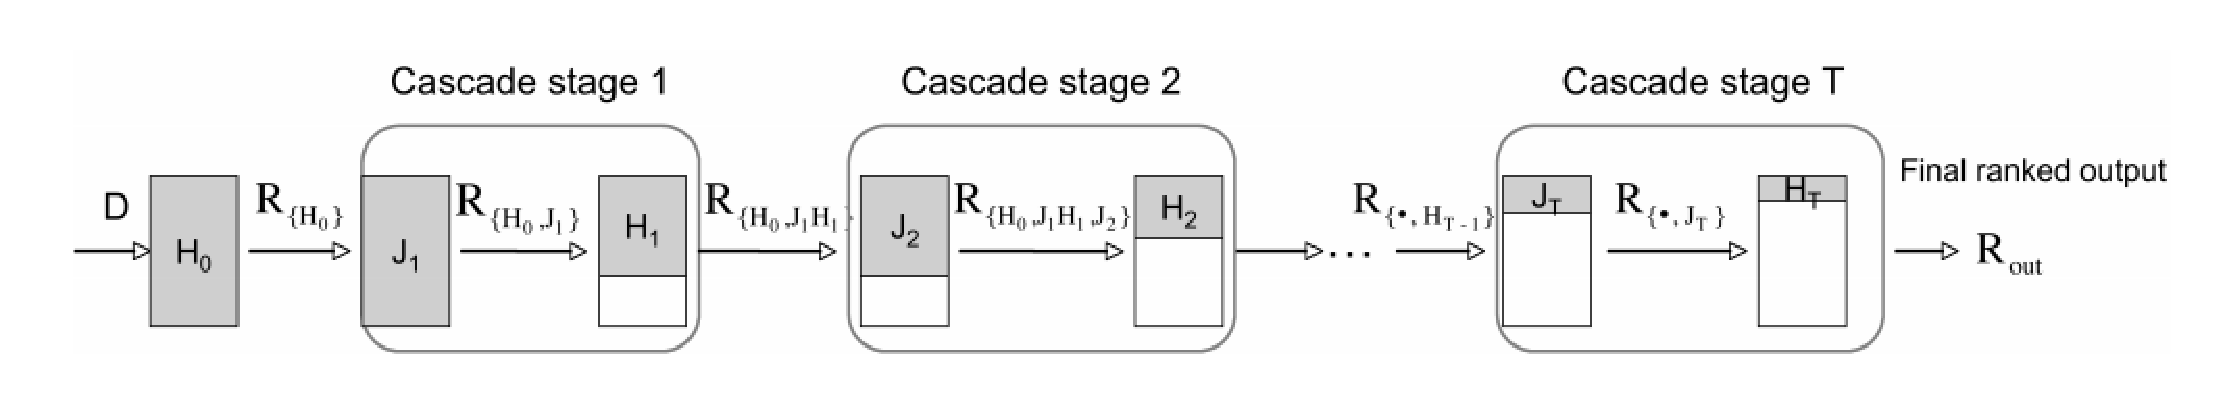
\includegraphics[width=0.9\textwidth]{figures/cascademodel.eps}
  \caption{级联模型}\label{fig:cascademodel}
\end{figure}

级联模型可以使用一组前后相继的阶段模型$\{\langle J_t(\beta_t), H_t, \alpha_t\rangle\}_{t=1}^T$来表示,每个阶段产生一个\textbf{完整的阶段模型},包括含参的剪枝模型$J_t(\beta_t)$、 弱排名函数$H_t$及其权值$\alpha_t$。为方便,记阶段$t$完整的阶段模型$S_t$:
\begin{equation}
    S_t = \langle J_t(\beta_t), H_t, \alpha_t\rangle
\end{equation}
在阶段$t$之前(包括阶段$t$)的所有阶段模型集合记为$G_t = \bigcup\limits_{i=0}^t S_i$。

\begin{algorithm}[htbp]
        \caption{级联排序算法}
        \begin{algorithmic}
            \REQUIRE ~~训练集$\{q_i,x_i,y_i\}^m_{i=1}$,级联阶数$T$,检索词概率分布$P_1(i)=1/m$,初始级联模型$G_0 =\varnothing$\\
            \FOR{$t = 1,\dots, T$}
            \STATE
            \begin{enumerate}
                \item 根据训练集检索词概率分布$P_t$,确定最佳的阶段模型$S_t = <J_t(\beta_t), H_t, \cdot>$:
                \begin{equation}
                    S_t = \argmin\limits_{S_t} \big[\eta_t^2 - \varphi_t^2\big]
                \end{equation}
                其中,%网格搜索(Grid Search)
                \begin{equation}
                    \left\{
                    \begin{array}{lll}
                      \eta_t & = & \sum\limits_{i=1}^m \frac{P_t(i)}{1-\gamma C(x_i,S_t)}\\
                      \varphi_t & = & \sum\limits_{i=1}^m \frac{P_t(i)}{1-\gamma C(x_i,S_t)} E(x_i,y_i,S_t)
                    \end{array}
                    \right.
                \end{equation}
                \item 给弱排名函数$H_t$赋最优权值$\alpha_t$:
                \begin{equation}
                    \alpha_t = \frac{1}{2} \log \frac{\eta_t + \varphi_t}{\eta_t - \varphi_t}
                \end{equation}
                \item 将完整的阶段模型$\langle J_t(\beta_t), H_t, \alpha_t\rangle$添加到$G_t$:
                \begin{equation}
                    G_t = G_{t-1} \cup \{\langle J_t(\beta_t), H_t, \alpha_t\rangle\}
                \end{equation}
                \item 根据级联模型在各个检索词上的表现,更新检索词的分布$P_{t+1}$:
                \begin{equation}
                    P_{t+1}(i)= \frac{\exp\{-E(x_i,y_i,f_t) + \gamma C(x_i,G_t)\}}{Z_t}
                \end{equation}
                其中,
                \begin{equation}
                    \left\{
                    \begin{array}{l}
                      f_t = \sum\limits_{k=1}^t \alpha_k H_k\\
                      E(x_i,y_i,f_t) = E(x_i,y_i,G_t)\\
                      Z_t = \sum\limits_{i=1}^{m} \exp\{-E(x_i,y_i,f_t) + \gamma C(x_i,G_t)\}
                    \end{array}
                    \right.
                \end{equation}
            \end{enumerate}
            \ENDFOR
            \ENSURE ~~最终排名函数$f_T = \sum\limits_{t=1}^{T}{\alpha_t H_t}$
        \end{algorithmic}
\end{algorithm}

级联排序问题属于多目标规划问题,为了兼顾模型效果与效率,级联模型定义了基于模型性能与计算开销的线性组合形式的\textbf{平衡度量指标(Tradeoff Metric)}:
\begin{equation}
    \mathrm{TM}_{ti} = E(x_i, y_i, G_t) - \gamma C(x_i, G_t)
\end{equation}
其中,$E(x_i,y_i,G_t)$表示直至阶段$t$的级联模型在检索词$q_i$上的排名效果,$C(x_i,G_t)$表示直至阶段$t$的级联模型的计算成本,$\gamma \in [0,1]$平衡两种指标对平衡度量指标的贡献,文中选择$\gamma = 0.1$。当$\gamma = 0$ 时,级联排序模型就简化成AdaRank模型,因此级联排序模型可以看做是AdaRank模型的推广。

成本函数$C(x_i, G_t)$一般可以使用下面的加和形式表示:
\begin{equation}
    C(x_i, G_t) = \sum\limits_{k=1}^t C(x_i, S_t)
\end{equation}
对于每个级联阶段,影响计算成本的因素包括排名模型$H_t$的复杂度,参与评估的文档数目,需要一种合适的成本估计方法。

通过对每个弱排名函数$H_t$(类似AdaRank,选择特征空间中的单个特征作为备选的弱排名函数)评估训练集中所有的检索词,并记录相应的时间开销,基于平均时间开销$U_t$ 估计计算成本:
\begin{equation}
    C(x_i, S_t) = U_t |R_{i\{\cdot, J_t\}}|
\end{equation}
其中,$|R_{i\{\cdot, J_t\}}|$表示参与评估的文档数目。为计算方便,作者选择衰减的指数函数$e^{-\delta C(x_i, G_t)}$,将计算成本映射到$[0,1]$区间,其中,$\delta  = 0.01$。

由此,可以定义下面形式的损失函数:
\begin{equation}
    \mathcal{L} = \frac{1}{m}\sum\limits_{i=1}^m \ell_i = \frac{1}{m} \sum\limits_{i=1}^m \exp \{ - E(x_i,y_i,G_t) + \gamma C(x_i,G_t)\})
\end{equation}

剪枝函数的作用是约减待评价的文档集,因为在实际应用中,多数文档属于不相关文档,那么预先将其从文档集中剔除,在提高文档整体质量的同时也提升了排名的效率。通常,剪枝函数都是含参$\beta_t$的评价准则,常用的剪枝函数有三种:
\begin{enumerate}
  \item 基于排名的剪枝函数(Rank-based):
  \[
    J_t(\beta_t) : \theta_t = (1-\beta_t) \times |R_{\{\cdot,H_{t-1}\}}|
  \]
  其中,$|R_{\{\cdot,H_{t-1}\}}|$表示在第$t$阶段输入的文档数目。这种剪枝函数要求对于排名低于$\theta_t$的文档剪枝。参数$\beta_t$越大,则剔除的文档越多(数值越小,名次越高)。
  \item 基于分值的剪枝函数(Score-based):
  \[
    J_t(\beta_t) : \theta_t = \beta_t \times [\max(R_{\{\cdot,H_{t-1}\}}) - \min(R_{\{\cdot,H_{t-1}\}})] + \min(R_{\{\cdot,H_{t-1}\}})
  \]
  其中,$max(R_{\{\cdot,H_{t-1}\}})$,$min(R_{\{\cdot,H_{t-1}\}})$表示$R_{\{\cdot,H_{t-1}\}}$中最大、最小的分值。如果文档的分值低于$\theta_t$,则从集合中剪除。
  \item 均值-最大值阈值准则(Mean-Max Threshold):
  \[
    J_t(\beta_t) : \theta_t = \beta_t \times \max(R_{\{\cdot,H_{t-1}\}}) + (1-\beta_t) \times \mathrm{mean}(R_{\{\cdot,H_{t-1}\}})
  \]
  其中,$\mathrm{mean}(R_{\{\cdot,H_{t-1}\}})$表示$R_{\{\cdot,H_{t-1}\}}$中文档的平均分值。如果待测文档分值低于$\theta_t$,则从集合中剪除。
\end{enumerate}

级联排序模型使用剪枝函数逐阶削减输入文档的数目,将相关性低的文档提前从输入集合中剔除,在提升训练效率的同时有助于改善文档集合的综合质量:
\begin{equation}
    \begin{array}{l}
      |R_{\{\cdot,J_t\}}| \le |R_{\{\cdot,J_{t-1}\}}| \le \cdots \le |R_{\{\cdot,J_1\}}|\\
      E(R_{\{\cdot,H_t\}}) \ge E(R_{\{\cdot,H_{t-1}\}}) \ge \cdots \ge E(R_{\{\cdot,H_0\}})
    \end{array}
\end{equation}
下面我们来证明级联排序模型具有持续改善排名性能的作用,证明步骤类似于AdaRank。

\begin{proof}
根据$\varphi_t, \eta_t, \alpha_t$的定义可知:
\begin{equation}
    e^{\alpha_t} = \sqrt{\frac{\eta_t + \varphi_t}{\eta_t - \varphi_t}}
\end{equation}

由于模型中用于衡量排序性能的指标$E\in [0,1]$,所以$e^{-E} \ge 1-E$,从而有:
\begin{equation}
    \begin{array}{lll}
      \frac{1}{m} \sum\limits_{i=1}^m \bigg[E(x_i, y_i, f_T) - \gamma C(x_i, G_T)\bigg] & \ge & \frac{1}{m} \sum\limits_{i=1}^m \bigg\{ 1 - exp\{-E(x_i, y_i, f_T) + \gamma C(x_i, G_T)\} \bigg\} \\
       & = & 1 - \frac{1}{m} \sum\limits_{i=1}^m exp\{-E(x_i, y_i, f_T) + \gamma C(x_i, G_T)\} \\
       & = & 1 - \frac{1}{m} Z_T
    \end{array}
\end{equation}
建立了模型平均性能指标同$Z_T$的关系,进而转向对$Z_T$上界的分析。

由于
\[
\begin{array}{lll}
      -E(x_i, y_i, f_T) + \gamma C(x_i, G_T) & = & \big[-E(x_i, y_i, f_T) + \alpha_T E(x_i, y_i, H_T) + E(x_i, y_i, f_{T-1})\big] \\
       & + & \big[- E(x_i, y_i, f_{T-1}) + \gamma C(x_i, G_{T-1}) \big]\\
       & + & \big[\gamma C(x_i, S_T) - \alpha_T E(x_i, y_i, H_T) \big]
\end{array}
\]
所以有:
\begin{equation}
    \begin{array}{lll}
      Z_T & = & \sum\limits_{i=1}^m exp\{-E(x_i, y_i, f_T) + \gamma C(x_i, G_T) \big]\} \\
       & = & \sum\limits_{i=1}^m \bigg[e^{-\delta_i^T} exp\{-E(x_i, y_i, f_{T-1}) + \gamma C(x_i, G_{T-1}\} exp\{\gamma C(x_i, S_T) - \alpha_T E(x_i, y_i, H_T)\} \bigg] \\
       & \le & e^{-\delta_{min}^T} Z_{T-1} \sum\limits_{i=1}^m \bigg[\frac{exp\{-E(x_i, y_i, f_{T-1}) + \gamma C(x_i, G_{T-1}\}}{Z_{T-1}} exp\{\gamma C(x_i, S_T) - \alpha_T E(x_i, y_i, H_T)\}\bigg] \\
       & = & e^{-\delta_{min}^T} Z_{T-1} \sum\limits_{i=1}^m P_T(i) exp\{\gamma C(x_i, S_T) - \alpha_T E(x_i, y_i, H_T)\} \\
       & \triangleq & e^{-\delta_{min}^T} Z_{T-1}  W_T
    \end{array}
\end{equation}
由于当$x>0$时,有$e^x \le \frac{1}{1-x}$,所以:
\begin{equation}
    e^{\gamma C(x_i, S_T)} \le \frac{1}{1 - \gamma C(x_i, S_T)}
\end{equation}
又因为:
\[
    -\alpha_T E(x_i, y_i, H_T) = \lambda (-\alpha_T) + (1-\lambda) \alpha_T
\]
其中,
\[
    \lambda = \frac{1+E(x_i,y_i,H_T)}{2}
\]
根据函数$f(x)=e^x$的凸性可知:
\begin{equation}
    e^{-\alpha_T E(x_i, y_i, H_T)} \le \frac{1+E(x_i,y_i,H_T)}{2} e^{-\alpha_T} + \frac{1-E(x_i,y_i,H_T)}{2} e^{\alpha_T}
\end{equation}

那么:
\begin{equation}
    \begin{array}{lll}
       W_T & = & \sum\limits_{i=1}^m P_T(i) exp\{\gamma C(x_i, S_T) -\alpha_T E(x_i, y_i, H_T)\} \\
       & \le & \sum\limits_{i=1}^m  \frac{P_T(i)}{1 - \gamma C(x_i, S_T)} e^{-\alpha_T E(x_i, y_i, H_T)} \\
       & \le & \sum\limits_{i=1}^m  \frac{P_T(i)}{1 - \gamma C(x_i, S_T)} \bigg\{\frac{1+E(x_i,y_i,H_T)}{2} e^{-\alpha_T} + \frac{1-E(x_i,y_i,H_T)}{2} e^{\alpha_T} \bigg\} \\
       & = & \sum\limits_{i=1}^m \frac{P_T(i)}{1 - \gamma C(x_i, S_T)} \bigg[ \frac{1+E(x_i,y_i,H_T)}{2}\bigg] e^{-\alpha_T} + \sum\limits_{i=1}^m \frac{P_T(i)}{1 - \gamma C(x_i, S_T)} \bigg[ \frac{1-E(x_i,y_i,H_T)}{2}\bigg] e^{\alpha_T}\\
       & = & \frac{\eta_T + \varphi_T}{2} e^{-\alpha_T} + \frac{\eta_T - \varphi_T}{2} e^{\alpha_T} \\
       & = & \sqrt{\eta_T^2 - \varphi_T^2}
    \end{array}
\end{equation}

从而可推知:
\begin{equation}
    \begin{array}{lll}
       Z_T & \le &  e^{-\delta_{min}^T} Z_{T-1} \sqrt{\eta_T^2 - \varphi_T^2}\\
       & = & Z_{T-2} \prod\limits_{t=T-1}^T e^{-\delta_{min}^t} \sqrt{\eta_t^2 - \varphi_t^2} \\
       & = & Z_1 \prod\limits_{t=2}^T e^{-\delta_{min}^t} \sqrt{\eta_t^2 - \varphi_t^2} \\
    \end{array}
\end{equation}

由于
\begin{equation}
    \begin{array}{lll}
      Z_1 & = & exp\{-E(x_i,y_i, \alpha_1 H_1) + \gamma C(x_i, G_1)\} \\
       & \le & e^{-\delta_{\min}^1} \sum\limits_{i=1}^m exp\{-\alpha_1 E(x_i,y_i, H_1) + \gamma C(x_i, S_1)\} \\
       & \le & e^{-\delta_{\min}^1} \sum\limits_{i=1}^m \frac{exp\{-\alpha_1 E(x_i,y_i, H_1)\}}{1-\gamma C(x_i, S_1)} \\
       & = & m \cdot e^{-\delta_{\min}^1} \big[e^{-\alpha_1} \sum\limits_{i=1}^m \frac{P_1(i)}{1-\gamma C(x_i, S_1)} \frac{1+E(x_i,y_i,H_1)}{2} + e^{\alpha_1} \sum\limits_{i=1}^m \frac{P_1(i)}{1-\gamma C(x_i, S_1)} \frac{1-E(x_i,y_i,H_1)}{2}\big]\\
       & = & m \cdot e^{-\delta_{\min}^1} \sqrt{\eta_1^2 - \varphi_1^2}
    \end{array}
\end{equation}

通过上面推导结果可知:
\begin{equation}
    Z_T \le m \prod\limits_{t=1}^T e^{-\delta_{\min}^t} \sqrt{\eta_t^2 - \varphi_t^2}
\end{equation}
因而可得:
\begin{equation}\label{eq:cascaderanktheorem}
    \frac{1}{m} \sum\limits_{i=1}^m \bigg[E(x_i, y_i, f_T) - \gamma C(x_i, G_T)\bigg] \ge 1- \prod\limits_{t=1}^T e^{-\delta_{\min}^T}  \sqrt{\eta_t^2 - \varphi_t^2},
\end{equation}
证毕。
\end{proof}

根据不等式\eqref{eq:cascaderanktheorem}可知,只要在每步迭代保证:
\[
    e^{-\delta_{\min}^t}  \sqrt{\eta_t^2 - \varphi_t^2} < 1
\]
成立,则排序模型的平均性能下界趋于上升,由此表明级联排名算法可以持续改善模型性能。

\section{排序逻辑回归模型}
2006年,Yan与Hauptmann~\cite{yan2006efficient}提出一种基于间隔(Margin-based)的广义排名学习框架,通过近似优化序对型风险函数估计模型参数,使用不同形式的损失函数与规则化项,可以推演出不同形式的排序模型,比如使用Logit 损失函数,他们提出了排序逻辑回归(Ranking Logistic Regression,RLR)模型,实验表明基于间隔的排序框架性能显著。

序对型排序学习方法将排名问题转化为二元分类问题,在分类框架下通过优化下面形式的正则化经验风险训练排序模型:
\begin{equation}
    \min\limits_{f} R_0(f) = \sum\limits_{q\in Q} \sum\limits_{i=1}^{n_q} L(y_i f(d_i,q)) + C\Omega(\|f\|_{\mathcal{H}})
\end{equation}
其中,第一部分是一般的经验风险,第二部分是正则化项。$Q$是检索词集合,$n_q$是同检索词$q$关联的文档数目,$y_i f(d_i,q)$是分类模型的“间隔”~\cite{hastie2009elements},$L$表示损失函数,一般地是关于间隔的递减函数,$\Omega$表示单调递增的规则化函数,$C>0$代表正则化系数。

分类框架下学习排序模型存在两个主要弊端,一方面模型预测精度对数据分布敏感,即某种类型的数据分布越多,则相应的预测结果就越倾向于此类型。另一方面,分类精度与排名精度不一致,模型分类精度很高,但是相应的排名性能未必尽如人意。为此,我们可以通过最大化同序对(Concordant Pairs)克服这些问题:
\begin{equation}
    \max\limits_f  \sum\limits_{q\in Q} \sum\limits_{d_i\in D_q^+} \sum\limits_{d_j\in D_q^-} I(f(d_i,q)>f(d_j,q))
\end{equation}

分析同序对可以发现,直接优化是行不通的,如果使用一个连续的、凸的、单调递减的损失函数替换它,势必可以方便模型优化工作。通过引入正则化项,本文给出下面统一形式的基于间隔的排序学习框架:
\begin{equation}
    \begin{array}{lll}
      \min\limits_{f} R_1(f) & = & \sum\limits_{q\in Q} \sum\limits_{d_i\in D_q^+} \sum\limits_{d_j\in D_q^-} L(f(d_i,q)-f(d_j,q)) + C\Omega(\|f\|_{\mathcal{H}}) \\
       & = & \sum\limits_{q\in Q} \sum\limits_{d_i\in D_q^+} \sum\limits_{d_j\in D_q^-} L(\sum\limits_{k=1}^n \omega_k[f_k(d_i,q) - f_k(d_j,q)]) + C\Omega(\|f\|_{\mathcal{H}})
    \end{array}
\end{equation}
排序模型选择最简单的线性模型$f(d,q) = \sum\limits_{k=1}^n \omega_k f_k(d,q)$,通过选择不同的损失函数与正则化项,就可以导出一系列排序模型。

\begin{definition}[排名一致性]
风险最小估计模型因子$\omega\in \mathbb{R}^n$,对任意的$d_i\in D_q^+,d_j\in D_q^-$,排名特征$f_k$如果满足$\omega_k(f_k(d_i,q) - f_k(d_j,q))\ge 0$,则称风险最小估计特征权值$\omega_k$与真实排名一致,我们称模型满足排名一致性(Rank Consistency)。
\end{definition}

\begin{theorem}
基于间隔的排序框架学习到的风险最小估计量$\omega_k$与真实排名一致。
\end{theorem}

\begin{proof}
如果存在排名特征$f_k$满足$f_k(d_i,q)\ge f_k(d_j,q),\forall q\in Q, d_i\in D_q^+,d_j\in D_q^-$,我们用反证法证明$\omega_k \ge 0$。 假设$\omega_k<0$,若记$\omega_k' = - \omega_k$,基于间隔的排序框架使用的损失函数是单调递减的,由于
\begin{equation}
    \omega_k (f_k(d_i,q) - f_k(d_j,q)) \le \omega_k'(f_k(d_i,q) - f_k(d_j,q))
\end{equation}
记$\Delta_k = \sum\limits_{l\ne k}  \omega_l(f_l(d_i,q) - f_l(d_j,q))$,则有
\begin{equation}
    L(\omega_k'(f_k(d_i,q) - f_k(d_j,q))+\Delta_k) \le L(\omega_k (f_k(d_i,q) - f_k(d_j,q)) + \Delta_k)
\end{equation}
这与$\omega_k$是风险最小估计量矛盾,故而$\omega_k\ge 0$。
\end{proof}

\begin{theorem}
若损失函数$L$是凸的,并且满足$2L(x/2)\ge L(x)$,则不等式成立:
\begin{equation}
    \frac{1}{2} \big[R_2(f) - R_2(-f)\big] \le R_1(f) \le R_2(f)
\end{equation}
其中,$R_1(f)$不含正则项,$R_2(f)$是一个基于有偏置的排名函数$f^b(d,q)$近似风险函数:
\begin{equation}
    R_2(f) = \sum\limits_{q\in Q} \bigg\{\sum\limits_{d_i\in D_q^+} |D_q^-| L(f^b(d_i,q)) + \sum\limits_{d_j\in D_q^-} |D_q^+| L(-f^b(d_j,q))\bigg\}
\end{equation}
其中,$|\cdot|$表示集合大小,$f^b(d,q) = \sum\limits_{k=1}^n \omega_k (f_k(d,q) - b_k)$。
\end{theorem}

\begin{proof}
由于损失函数是凸的并且$2L(x/2)\ge L(x)$,则对任意的$A,B\in \mathbb{R}$,都有
\[
    L(A) + L(B) \ge 2L(\frac{A+B}{2})\ge L(A+B)
\]
类似地可得
\[
    L(A+B) + L(-B) \ge 2L(\frac{A}{2})\ge L(A), L(A+B) + L(-A) \ge L(B)
\]
将两个不等式相加有:
\[
    2L(A+B) + L(-B) + L(-A) \ge L(A) + L(B)
\]
整理可得$L(A+B) \ge \frac{1}{2} \big[L(A) + L(B) - L(-A) - L(-B)\big]$,综上:
\begin{equation}
    L(A) + L(B) \ge L(A+B) \ge \frac{1}{2} \big[L(A) + L(B) - L(-A) - L(-B)\big]
\end{equation}

令$A=f^b(d_i,q),B=-f^b(d_j,q)$,我们有
\begin{equation}
    \begin{array}{lll}
      L(f^b(d_i,q)) + L(-f^b(d_j,q)) & \ge & L(f^b(d_i,q)-f^b(d_j,q)) = L(f(d_i,q)-f(d_j,q))\\
       & \ge & \frac{1}{2} \big[L(f^b(d_i,q)) + L(-f^b(d_j,q)) - L(-f^b(d_i,q)) - L(f^b(d_j,q))\big]
    \end{array}
\end{equation}
两边同时加和
\begin{equation}
    \begin{array}{ll}
       & \sum\limits_{q\in Q} \sum\limits_{d_i\in D_q^+} \sum\limits_{d_j\in D_q^-} \big[L(f^b(d_i,q)) + L(-f^b(d_j,q))\big]\\
       \ge & \sum\limits_{q\in Q} \sum\limits_{d_i\in D_q^+} \sum\limits_{d_j\in D_q^-} L(f(d_i,q)-f(d_j,q))\\
       \ge & \frac{1}{2} \sum\limits_{q\in Q} \sum\limits_{d_i\in D_q^+} \sum\limits_{d_j\in D_q^-} \big[L(f^b(d_i,q)) + L(-f^b(d_j,q)) - L(-f^b(d_i,q)) - L(f^b(d_j,q))\big]
    \end{array}
\end{equation}
由于第一个不等式
\begin{equation}
    \begin{array}{ll}
        & \sum\limits_{q\in Q} \sum\limits_{d_i\in D_q^+} \sum\limits_{d_j\in D_q^-} \big[L(f^b(d_i,q)) + L(-f^b(d_j,q))\big] \\
      = & \sum\limits_{q\in Q} \big\{\sum\limits_{d_i\in D_q^+}|D_q^-| L(f^b(d_i,q))+\sum\limits_{d_j\in D_q^-}|D_q^+|L(-f^b(d_j,q))\big\} \\
      = & R_2(f)
    \end{array}
\end{equation}
因此可得第二个不等式
\begin{equation}
    \begin{array}{ll}
        & \frac{1}{2} \sum\limits_{q\in Q} \sum\limits_{d_i\in D_q^+} \sum\limits_{d_j\in D_q^-} \big[L(f^b(d_i,q)) + L(-f^b(d_j,q)) - L(-f^b(d_i,q)) - L(f^b(d_j,q))\big] \\
      = & \frac{1}{2} \big[R_2(f) - R_2(-f)\big] \\
    \end{array}
\end{equation}
综上有$\frac{1}{2} \big[R_2(f) - R_2(-f)\big] \le R_1(f) \le R_2(f)$。特别地,如果$L$是线性的,则等式成立。
\end{proof}

近似风险函数$R_2(f)$的计算复杂度是$\complex(|D_q^+| + |D_q^-|)$远低于$R_1(f)$的复杂度$\complex(|D_q^+||D_q^-|)$,此外通过系数$|D_q^+|,|D_q^-|$ 抵消两类数据分布不平衡的影响,最大化两类数据的预测间隔。

如果取Logit损失函数
\begin{equation}
    L(x) = \log(1+e^{-x})
\end{equation}
那么有
\[
    L(x) + L(-x) = \log(1+e^{-x}) + \log(1+e^{x}) \le 2 + |x|
\]

在模型训练之前,必须首先确定偏置向量$b$,为此,可通过最小化上下界之差
\begin{equation}
    b^* = \argmin\limits_b \frac{1}{2} \big[ R_2(f) + R_2(-f)\big]
\end{equation}
使近似风险函数$R_2$更贴近于$R_1$的准确值,由于
\begin{equation}
    \frac{1}{2} \big[ R_2(f) + R_2(-f)\big] \le 2|Q||D_q^+||D_q^-| + \frac{1}{2} \sum\limits_{q\in Q} \bigg\{\sum\limits_{d_i\in D_q^+} |D_q^-| |f^b(d_i,q)|  + \sum\limits_{d_j\in D_q^-} |D_q^+| |f^b(d_j,q)|\bigg\}
\end{equation}
偏置向量的优化等价于下面的优化问题
\begin{equation}
    \min\limits_b \sum\limits_{q\in Q} \bigg\{\sum\limits_{d_i\in D_q^+} |D_q^-| |f^b(d_i,q)|  + \sum\limits_{d_j\in D_q^-} |D_q^+| |f^b(d_j,q)|\bigg\}
\end{equation}
直接优化难以实现,为此,使用一组优化模型逐个优选偏置量,达到近似优化的目的:
\begin{equation}
    \min\limits_{b_k} \sum\limits_{q\in Q}\bigg\{\sum\limits_{d_i\in D_q^+} |D_q^-| |f_k(d_i,q) - b_k|  + \sum\limits_{d_j\in D_q^-} |D_q^+| |f_k(d_j,q) - b_k|\bigg\}
\end{equation}
最优的偏置量是同一个排名特征下,所有检索词关联文档特征值的中值:
\begin{equation}
    \omega_k^* = \mathrm{median}\bigg\{\bigcup\limits_{q \in Q} \bigg(\bigcup\limits_{d_i \in D_q^+} \big\{f_k(d_i,q)\big\}_{|D_q^-|} \bigcup \bigcup\limits_{d_j \in D_q^-} \big\{f_k(d_j,q)\big\}_{|D_q^+|} \bigg)\bigg\}
\end{equation}
其中,$\{x\}_n$表示$n$个数值都等于$x$的集合,等价于将每个排名特征中值都转化为0。

将最优的偏置向量代入至$R_2(f)$中,使用Logit损失函数与$\ell_2$规则化项,我们可以利用梯度下降法进行优化。

\section{序对协调排名方法}
假设检索词$q$的关联文档集合是$\{x_i,r_i\}_{i=1}^n$,利用训练集学习线性模型$f(\omega,x)=\omega^T x$,我们要求模型在单个文档、文档序对及文档序列层面具有下面三条性质:
\begin{enumerate}
  \item 逐点型:预测结果与真实相关等级之间的误差尽可能小
  \[
    \argmin\limits_{\omega}~\sum\limits_{i=1}^n \|\omega^T x_i - r_i\|
  \]
  \item 序对型:对于检索词$q$的任意两个关联文档$x_i,x_j$,基于预测分值的排名结果与真实排名一致
  \[
    (\omega^T x_i - \omega^T x_j)(r_i - r_j) = \omega^T (x_i - x_j)(r_i - r_j) \ge 0
  \]
  \item 序列型:在检索词$q$上的排名精度尽可能高
  \[
    \argmax\limits_{\omega}~E(q,f)
  \]
  其中,$E$表示衡量排序性能的标准指标,如MAP、NDCG等。
\end{enumerate}

\textbf{序对型约束条件}要求预测模型能够最大化\textbf{序对间隔},由此建立下面形式的优化问题
\[
  \max\limits_{\omega} ~~\sum\limits_{(i,j)} \omega^T (x_i - x_j)(r_i - r_j)
\]
由于
\[
    (x_i - x_j)(r_i - r_j) = (x_j - x_i)(r_j - r_i)
\]
则原始问题等价于下面形式的优化问题
\begin{equation}\label{eq:clr}
  \max\limits_{\omega} ~~\sum\limits_{(i,j) \in \mathscr P} \omega^T (x_i - x_j)(r_i - r_j)
\end{equation}
其中,集合$\mathscr P$表示文档偏好序对集,定义为
\[
   \mathscr P = \{(i,j)\mid r_i > r_j, i,j = 1,\ldots, n\}
\]
对同序对间隔项进行整理,可得:
\begin{equation}\label{eq:concordantmargin}
 \begin{array}{ll}
    & \sum\limits_{(i,j) \in \mathscr P} (x_i - x_j)(r_i - r_j) \\
    = & \sum\limits_{(i,j) \in \mathscr P} \bigg[ x_i(r_i - r_j) - x_j(r_i - r_j)\bigg] \\
    = & \sum\limits_{i=1}^n x_i \sum\limits_{j\in \mathscr P_{i*}} (r_i - r_j) + \sum\limits_{j=1}^n x_i \sum\limits_{i\in \mathscr P_{*j}} (r_i - r_j) \\
    = & \sum\limits_{i=1}^n x_i \sum\limits_{j\in \mathscr P_{i*}\bigcup \mathscr P_{*i}} (r_i - r_j)\\
    \equiv & \sum\limits_{i=1}^n x_i \alpha_i
 \end{array}
\end{equation}
其中,集合
\[
    \mathscr P_{i*} = \{j\mid (i,j)\in \mathscr P, \forall j=1,\ldots,n\},~~\mathscr P_{*i} = \{j\mid (j,i)\in \mathscr P, \forall j=1,\ldots,n\}
\]
是根据样本$i$的相关等级对样本集合做出的一种,前者是所有等级低于$i$的样本集合,后者是所有等级高于$i$的样本集合。此外,还有一部分样本,它们的等级与样本$i$的相同,记为$\mathbb{S}_r$:
\begin{equation}
    \mathbb{S}_r = \{i\mid r_i = r, \forall i=1,\ldots,n\}, \forall r\in \mathbb{G}
\end{equation}
其中,样本$i$的相关等级等于$r$,$\mathbb{G}$表示数据集上所有相关等级的集合。

序对协调排名方法(Pairwise Concordant Ranking Method,PCRank)在优化问题\eqref{eq:clr}之上添加一个规则化项:
\begin{equation}
    L(\omega, \lambda) = \omega^T \sum\limits_{i=1}^n x_i \alpha_i - \frac{\lambda}{2} \| \omega \|^2
\end{equation}
若取$\ell_2-$范数,由极值必要性条件可知
\begin{equation}
    \omega^* = \frac{1}{\lambda} \sum\limits_{i=1}^n x_i \alpha_i
\end{equation}
其中,$\omega^*$是最优解,在不产生混淆的情况下,我们略去上标星号。由于$\lambda>0$,不会影响预测的排名结果,等价于
\begin{equation}
    \omega = \sum\limits_{i=1}^n x_i \alpha_i
\end{equation}
其中,$X\in\mathbb{R}^{n\times m}$表示训练数据集,每行表示一个数据样本特征向量。

我们利用等价关系
\[
    \mathscr P_{i*} \cup \mathscr P_{*i} = \{1,\ldots,n\}\backslash \mathbb{S}_r
\]
进一步化简等式\eqref{eq:concordantmargin},可得
\begin{equation}
 \begin{array}{lll}
    \omega & = & \sum\limits_{i=1}^n x_i \alpha_i \\
    & = & \sum\limits_{i=1}^n x_i \sum\limits_{j\in \mathscr P_{i*} \cup \mathscr P_{*i}} (r_i - r_j)\\
    & = & \sum\limits_{r\in \mathbb{G}} \sum\limits_{j\notin \mathbb{S}_r} (r - r_j) \sum\limits_{i\in \mathbb{S}_r} x_i\\
    & = & \sum\limits_{r\in \mathbb{G}} [(n - |\mathbb{S}_r|)r -\sum\limits_{j\notin \mathbb{S}_r} r_j] \sum\limits_{i\in \mathbb{S}_r} x_i\\
    & = & \sum\limits_{r\in \mathbb{G}} [nr - \sum\limits_{r_0\in \mathbb{G}} r_0|\mathbb{S}_{r_0}|] \sum\limits_{i\in \mathbb{S}_r} x_i \\
    & \equiv & \sum\limits_{r\in \mathbb{G}} (\beta_r \sum\limits_{i\in \mathbb{S}_r} x_i)
 \end{array}
\end{equation}
当$r$是最小的相关等级,则必然有$\beta_r\le 0$;反之,当$r$是最大的相关等级,则必然有$\beta_r>0$。如果训练数据只包含一种相关等级,则$\omega=0$。

若数据集线性不可分,引入核函数$K$则有:
\begin{equation}
    \begin{array}{lll}
      \omega^T \phi(x) & = & \sum\limits_{r\in \mathbb{G}} [nr - \sum\limits_{r_0\in \mathbb{G}} r_0|\mathbb{S}_{r_0}|] \sum\limits_{i\in \mathbb{S}_r} \phi(x_i)^T \phi(x) \\
      & = & \sum\limits_{r\in \mathbb{G}} [nr - \sum\limits_{r_0\in \mathbb{G}} r_0|\mathbb{S}_{r_0}|] \sum\limits_{i\in \mathbb{S}_r} K(x_i,x)
    \end{array}
\end{equation}
其中,$\phi$是映射函数,将输入变量映射到再生核Hilbert特征空间。\textcolor{blue}{基于核函数的PCRank存在一个严重的问题,在模型预测时所有的训练样本输入特征都要参与计算,无疑是不可行的。我们可以根据每个相关等级(或类别)下的输入特征,确定输入特征向量各个维度的区间范围,使用特征边界建立预测模型。}

利用相关等级可将关联文档集合划分成多个等价类,统计各个等价类下样本个数$|\mathbb{S}_{r_0}|$,只需复杂度为$\complex(n)$的时间就可以迅速确定对应与检索词$q$的最佳线性模型。我们使用此办法,对不同检索词构建不同的线性模型,作为基本排名函数,使用AdaRank算法,基于Boosting技术集成为强排名函数。

在确定最佳基本线性模型时,模型参数(特征权值)可能存在负值,并且对各个等级相关文档分布十分敏感。对于同一组数据集,相关等级经过保序变换,本质上并不会影响预测模型的排名精度。本模型可能会受到相关等级保序变换的影响,我们下面考察保序变换对线性模型的影响(假设相关等级保序变换函数为$\psi$):
\begin{equation}
    \begin{array}{lll}
      \beta_r \sum\limits_{i\in \mathbb{S}_r} x_i & = & nr - \sum\limits_{r_0\in \mathbb{G}} r_0|\mathbb{S}_{r_0}| \sum\limits_{i\in \mathbb{S}_r} x_i\\
      & = & \sum\limits_{r_0\in \mathbb{G}} |\mathbb{S}_{r_0}| (r-r_0) \sum\limits_{i\in \mathbb{S}_r} x_i\\
      & = & \sum\limits_{r_0\in \mathbb{G}} |\mathbb{S}_r| |\mathbb{S}_{r_0}| (r-r_0) \sum\limits_{i\in \mathbb{S}_r} x_i/ |\mathbb{S}_r|\\
      & = & \bar{x}_r \sum\limits_{r_0\in \mathbb{G}} |\mathbb{S}_r| |\mathbb{S}_{r_0}| (r-r_0)
    \end{array}
\end{equation}
因此,$\beta$可以看做是每个相关等级所有文档特征向量加权平均值权重。

相关等级进行线性变换$\psi(r) = a*r+b$
\begin{equation}
    \beta_r' \sum\limits_{i\in \mathbb{S}_r} x_i = \bar{x}_r \sum\limits_{r_0\in \mathbb{G}} |\mathbb{S}_r| |\mathbb{S}_{r_0}| [\psi(r) - \psi(r_0)] = a \beta_r \sum\limits_{i\in \mathbb{S}_r} x_i
\end{equation}
对关联文档的排名不会产生任何影响。

在PCRank模型中,相同等级的文档序对Pairwise Concordance间隔无任何贡献。分析模型的预测精度可以发现,相同等级的文档预测结果越接近则模型预测精度越高
\begin{equation}
    \min\limits_{\omega} ~\sum\limits_{r\in \mathbb{G}} \sum\limits_{i,j\in \mathbb{S}_r} |\omega^T x_i - \omega^T x_j|
\end{equation}
并且对于等级越高的文档序对,它们的预测接近程度更有利于提升模型整体的预测精度,为此可以添加权重因子
\begin{equation}
    \max\limits_{\omega} ~\sum\limits_{r\in \mathbb{G}} \sum\limits_{i,j\in \mathbb{S}_r} \varphi(r) |\omega^T x_i - \omega^T x_j|
\end{equation}
由于在文档标记中,相关等级数值越小则等级越高,则$\varphi(r)$是关于相关等级的单调递减函数,比如$\varphi(r)=e^{-r}$。

将相同等级的文档序对预测结果接近程度添加到PCRank模型中,建立下面形式的模型(统一称为PCRank模型)
\begin{equation}
    \max\limits_{\omega} ~ \sum\limits_{(i,j)\in \mathscr P} (\omega^T x_i - \omega^T x_j) [\psi(r_i)-\psi(r_j)] - \gamma \sum\limits_{r\in \mathbb{G}} \sum\limits_{i, j\in \mathbb{S}_r} \varphi(r) |\omega^T x_i - \omega^T x_j| - \frac{1}{2} \lambda \|\omega\|^2
\end{equation}
其中,$\lambda>0$,函数$\psi$是关于相关等级$r$的单调递增函数,提升模型在高相关等级文档上的预测精度,$\gamma>0$可以融入到单调递减函数$\varphi$ 中。

\textcolor{blue}{
假设预测函数为$f$,一般性的PCRank模型可以表示如下
\begin{equation}
    \max\limits_{f\in \mathcal H} ~ J(\theta,\lambda) = \sum\limits_{(i,j)\in \mathscr P} \big[f(x_i) - f(x_j)\big] [\psi(r_i)-\psi(r_j)] - \sum\limits_{r\in \mathbb G} \sum\limits_{i, j\in \mathbb{S}_r} \varphi(r) \big|f(x_i) - f(x_j)\big| - \frac{1}{2} \lambda \|f\|_\mathcal{H}^2
\end{equation}
}
模型反映了聚类的部分思想:使不同类别的样本数据尽量分散,相同类别的样本数据尽量聚集,并保证预测结果与真实相关等级的一致性。PCRank模型可以应用到多元分类问题

PCRank模型可以应用到分类问题:选择最优的阈值$b$(每个分类一个阈值),确保分类误差最小:
\begin{equation}
    \argmax\limits_{b} ~\sum\limits_{r\in \mathbb{G}} \sum\limits_{i\in \mathbb{S}_r} I(g(\omega^T x_i + b_r) = y_i)
\end{equation}

\section{公开数据集:排序学习}
排序学习是典型的监督学习方法,使用包含人工标记的数据作为训练数据集训练模型。目前,支持排序学习训练、检测的数据集很多,比如微软亚洲研究院提供的LETOR\cite{qin2010letor}、Microsoft Learning to Rank、Yahoo! Learning to Rank Challenge、Yandex Internet Mathematics等。

\subsection{LETOR}
目前,LETOR
\footnote{LETOR: \href{http://research.microsoft.com/en-us/um/beijing/projects/letor/}{http://research.microsoft.com/}}
公开数据集是排序学习研究人员使用最多的标准数据集,并且还提供多种经典排序学习算法的实验结果。LETOR是\textbf{LE}arning \textbf{TO} \textbf{R}ank的缩写,由微软亚洲研究院(Microsoft Research Asia,MSRA)发布。从2007年4月至2009年7月,MSRA已经发布了四个版本,本文实验使用的数据集是LETOR 3.0与LETOR 4.0两个版本。本节主要介绍实验中使用的LETOR数据集基本信息。

LETOR数据集包含的数据信息有三个主要部分:检索词集合、文档集合(也称“语料库”)、文档与检索词的相关等级。检索词集合与文档集合来源不同,前者统一标记赋予唯一的ID号,后者源自于网络采集程序从互联网上抓取的网页数据,并且以数值型的文档特征向量形式存储。文档与检索词的相关等级是监督学习的“标准答案”,部分来自于人工标记,还有是根据Bing搜索引擎的搜索日志生成。在LETOR 3.0数据包中含有七个数据集:HP2003、HP2004、NP2003、NP2004、TD2003、TD2004 和OHSUMED,LETOR 4.0 则含有两个数据集:MQ2007与MQ2008。

LETOR 3.0使用的文档集合是OHSUMED和Gov语料库。OHSUMED语料库\cite{hersh1994ohsumed}属于医学文献数据库MEDLINE的一个数据集,由1987年至1991年刊发的、出自270 个医学期刊的348,566篇医学文献构成。OHSUMED数据集由106个检索词,大约16,140篇文档构成,每篇文档提取45个特征,并根据文档与检索词的相关程度标记为三个等级:高度相关、部分相关、不相关。Gov语料库包含大约1,053,110篇网页,是2002年初从域名后缀为.gov的政府网站上爬取下来的。2003年,Gov语料库开始用于文本检索会议(Text REtrieval Conference,TREC)Web检索项目\cite{craswell2003overview}下的主题提取(Topic Distillation,TD)、主页发现(Home Page Finding,HP)和命名网页发现(Named Page Finding,NP)三类检索任务,语料库中每篇网页提取64个特征,文档与检索词的相关性标记为两个等级:相关与不相关。2003年、2004年文本检索会议Web 检索项目使用的数据集有六组:TD2003,TD2004,HP2003,HP2004,NP2003,NP2004。LETOR 4.0使用的文档集合是Gov2语料库、使用的检索词集合源自2007 年、2008 年文本检索会议Million Query(MQ)项目,分别记为MQ2007与MQ2008。Gov2语料库源自2004年初从政府网站上爬取下来的25,000,000篇网页,达到426G。语料库中每篇网页提取46个特征。MQ2007、MQ2008分别包含1700条、800条检索词。每个检索词文档,所有训练数据标记为三个等级:高度相关、相关、不相关。

\subsection{Microsoft Learning to Rank}
数据集采自Bing的标签集合,相关等级有5个级别:0(不相关)$\sim$ 4(完全相关)。它包含两组数据集:MSLR-WEB30k、MSLR-WEB10k,前者包含30,000个检索词,后者只有10,000检索词。每对query-doc包含136个特征。

\subsection{Yahoo! Learning to Rank Challenge}
Yahoo! 实验室于2010年初举办了一次Learning to Rank 挑战赛
\footnote{\href{http://webscope.sandbox.yahoo.com/catalog.php?datatype=c}{Yahoo! Learning to Rank Challenge}}
,使用的数据源自Yahoo!自己用作训练排名函数的子数据集。它包含两组数据集,一大一小,分别被分割成三个子数据集:训练集、验证集、测试集。数据包含700个特征,评价分5个等级:0(不相关)$\sim$ 4(高度相关)。\cite{chapelle2011yahoo}总结了竞赛的结果,并对胜出模型做出评价。

\subsection{Yandex Internet Mathematics}
Yandex是俄罗斯目前最大的搜索引擎公司,于2009年组织了一场互联网数学竞赛(Internet Mathematics Challenge)
\footnote{Internet Mathematics Challenge: \href{http://imat2009.yandex.ru/en}{2009}, \href{http://imat-relpred.yandex.ru/en}{2011}}
,竞赛使用的数据分成两部分:训练集与测试集。训练集中包含9,124条检索词,97,290篇文档。测试集总共包含115,643篇文档,取出21,103篇文档作为公开测试数据,其他用作最终测试。每篇文档提取245个特征,训练数据由人工标记为5个等级(0$\sim$4)。


\section{排序学习算法汇总表}
\begin{table}[ht]
\centering
    \begin{tabular}{|l|l|l|l|l|l|l|}
      \hline
      类型 & 名称 & 时间 & 损失函数 & 优化方法 & 数据集 & 对比算法\\
      \hline
      SVM & RankSVM\cite{joachims2002optimizing} &2002 & & & &\\
      SVM & IR-SVM\cite{cao2006adapting} & 2006& & & &\\
      SVM & SVM\textsuperscript{MAP}\cite{yue2007support} &2007 & & & &\\
      \hline
      ANN & PRank\cite{crammer2001pranking} & 2001 & & & &\\
      ANN & RankNet\cite{burges2005learning} & 2005 & & & &\\
      ANN & LambdaRank\cite{burges2007learning} & 2007 & & & &\\
      ANN & LambdaMART\cite{burges2010from} & 2010 & & & &\\
      ANN & ListNet\cite{cao2007learning} & 2007 & & & &\\
      ANN & ListMLE\cite{xia2008listwise} & 2008 & & & &\\
      ANN & QBRank\cite{zheng2007general}& 2007 & & & &\\
      ANN & FRank\cite{tsai2007frank}& 2007 & & & &\\
      ANN & SortRank\cite{rigutini2008sortnet}& 2008 & & & &\\
      ANN & BoltzRank\cite{volkovs2009boltzrank}& 2009 & & & &\\
      \hline
      Boosting & RankBoost\cite{freund2003efficient} & 2003& & & &\\
      Boosting & AdaRank\cite{xu2007adarank} & 2007& & & &\\
      Boosting & RankCosine\cite{qin2008query} & 2008& & & &\\
      Boosting & SRankBoost\cite{amini2008boosting} & 2008 & & & &\\
      Boosting & NDCGBoost\cite{valizadegan2009learning} & & & & &\\
      Boosting & GBRank\cite{zheng2007regression} & 2007 & & & &\\
      Boosting & RankRefine\cite{jin2008ranking} & & & & &\\
      Boosting & MPBoost\cite{zhu2009general} & & & & &\\
      Boosting & GBlend\cite{chen2010learning}& 2010 & & & &\\
      \hline
      Regression & SLR\cite{cooper1992probabilistic} & 1992 & & & &\\
      Regression & RankLR\cite{sculley2009large} & 2009 & & & &\\
      Regression & CRR\cite{sculley2010combined} & 2010 & Combined & SGD & &\\
      Regression & IntervalRank\cite{moon2010intervalrank} & 2010 & & & &\\
      -- & RankGP\cite{yeh2007learning} & 2007 & & GA & &\\
      -- & McRank\cite{li2007mcrank} & 2007 & & & &\\
      -- & SoftRank\cite{taylor2008softrank} & 2008 & & &\\
      -- & RankRLS\cite{pahikkala2009efficient}  & 2009 & & & &\\
      Bayes & BayesRank\cite{kuo2009learning}  & 2009 & & & &\\
      -- & PermuRank\cite{xu2008directly} & 2008& & & &\\
      \hline
    \end{tabular}
\end{table}
